\chapter{Vectors and Geometry}

%%%%%%%%%%%%%%%%%%%%%%%%%%%%%%%%%%%%%%%%%%%%%%%%%%%%%%%%%%%%%%%%%%%%%%%%%%%%

\section{Chapter Introduction}

This chapter contains an introduction to vectors, which correspond to
points in two, three and higher dimensional spaces. In this chapter,
you will become familiar with basic vector operations such as
addition, scalar multiplication, length, the dot product, and the
cross product (for three dimensional vectors). Vector representation
of lines in 2D and 3D and planes in 3D are presented. Criteria for when
such objects intersect at unique points is given in terms of
determinants. This geometric presentation motivates our study of these
kind of problems in higher dimensional settings in later
chapters. Throughout this chapter, MATLAB commands are introduced that
perform the operations described in the text. For 2D and 3D problems,
using MATLAB is only a convenience. For higher dimensions, doing the
computations by hand (even with a calculator) is impractical, and a
computational framework like MATLAB is essential to be able to solve
these problems.

%%%%%%%%%%%%%%%%%%%%%%%%%%%%%%%%%%%%%%%%%%%%%%%%%%%%%%%%%%%%%%%%%%%%%%%%%%%%

\section{Vectors}

Vectors are used to describe quantities that have both a magnitude and
a direction. You are probably familiar with vector quantities in two
and three dimensions, such as forces and velocities.

Later in this course we will see that vectors can also describe the
configuration of a mechanical system of weights and springs, or the
collections of voltages and currents in an electrical circuit.  These
more abstract vector quantities are not so easily visualized since
they take values in higher dimensional spaces.

We begin this course by discussing the geometry of vectors in two and
three dimensions.  In two and three dimensions, vectors can be
visualized as arrows. Before we can draw a vector, we have to decide
where to place the tail of the vector.  If we are drawing forces, we
usually put the tail of the vector at the place where the force is
applied. For example, in Figure~\ref{fig_pend} (left) 
the forces acting on a pendulum
bob are gravity and the restraining force along the shaft.

\begin{figure}
\centerline{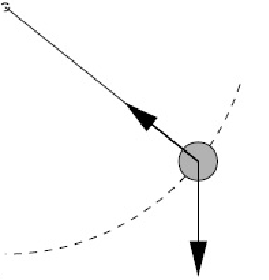
\includegraphics[height=1.5in]{2_pend}
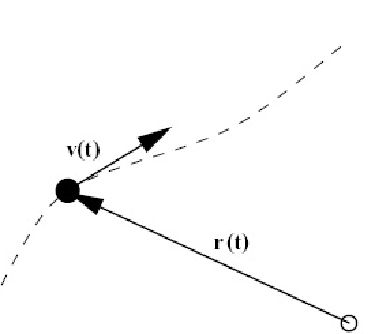
\includegraphics[height=1.5in]{2_velocity}}
\caption{Forces acting on a pendulum (left) and 
position and velocity of a particle (right) \label{fig_pend}}
\end{figure}

If we are drawing the velocity of a particle at a given time, we would
place the tail of the velocity vector ${\bf v}(t)$ at the position of
the particle at that time as shown in Figure~\ref{fig_pend} (right). 
Once we have chosen a starting point for the tails of our vectors
(i.e., an origin for space), every point in space corresponds to
exactly one vector, namely the vector whose tail is at the origin and
whose head is at the given point. For example, in Figure~\ref{fig_pend} 
(right)
we have chosen an arbitrary point as the origin (marked with a circle)
and identified the position of the particle with the vector ${\bf
r}(t)$.

\subsection{Multiplication by a number and vector addition}

There are two basic operations defined for vectors. One is
multiplication of a vector by a number (also called scalar
multiplication). The other is addition of two vectors.

A vector $\aa$ can be multiplied by a number (or scalar) $s$ to
produce a new vector $s\aa$. If $s$ is positive then $s\aa$ points in
the same direction as $\aa$ and has length $s$ times the length of
$\aa$. This is shown in Figure~\ref{fig_scalarmult}.
If $s$ is negative then $s\aa$ points in the direction opposite
to $\aa$ and has length $|s|$ times the length of $\aa$.

\begin{figure}
\centerline{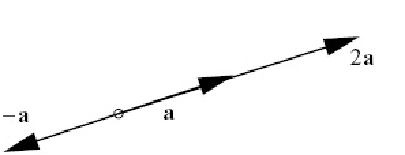
\includegraphics[height=1.5in]{2_scalarmult}}
\caption{Scalar multiplication. \label{fig_scalarmult}}
\end{figure}

To add two vectors $\aa$ and $\bb$ and we draw the parallelogram that
has $\aa$ and $\bb$ as two of its sides as shown in Figure~\ref{fig_add}. 
The vector $\aa + \bb$ has
its tail at the origin and its head at the vertex of the parallelogram
opposite the origin. Alternatively we can imagine sliding (or
translating) one of the vectors, without changing its direction, so
that its tail sits on the head of the other vector. (In the diagram we
translated the vector $\aa$.) The sum $\aa + \bb$ is then the vector
whose tail is at the origin and whose head coincides with the vector
we moved.

\begin{figure}
\centerline{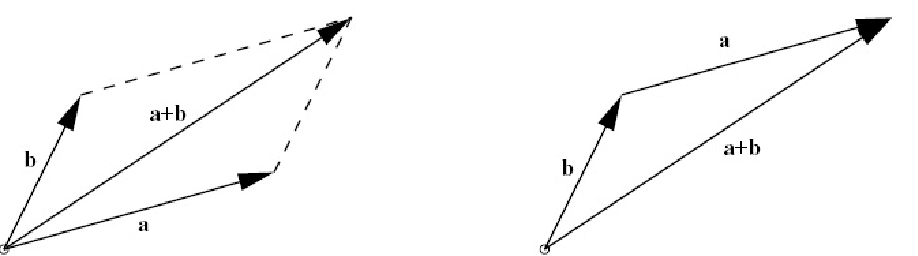
\includegraphics[height=1.5in]{2_add}}
\caption{Vector Addition. \label{fig_add}}
\end{figure}

\begin{example}
\label{2009_a1_3}
Describe and sketch the following set of points $\{ s {\bf a} :
s \in \mathbb{R} \}$ (that is, the set of all scalar multiples of $\bf a$) where
$\bf a$ is a non-zero vector in $\mathbb{R}^2$. {\rm The set is a straight line 
going through the origin with direction $\bf a$ as shown in 
Figure~\ref{ch2exnew1}.}
\end{example}

\begin{figure}[htb]
\centerline{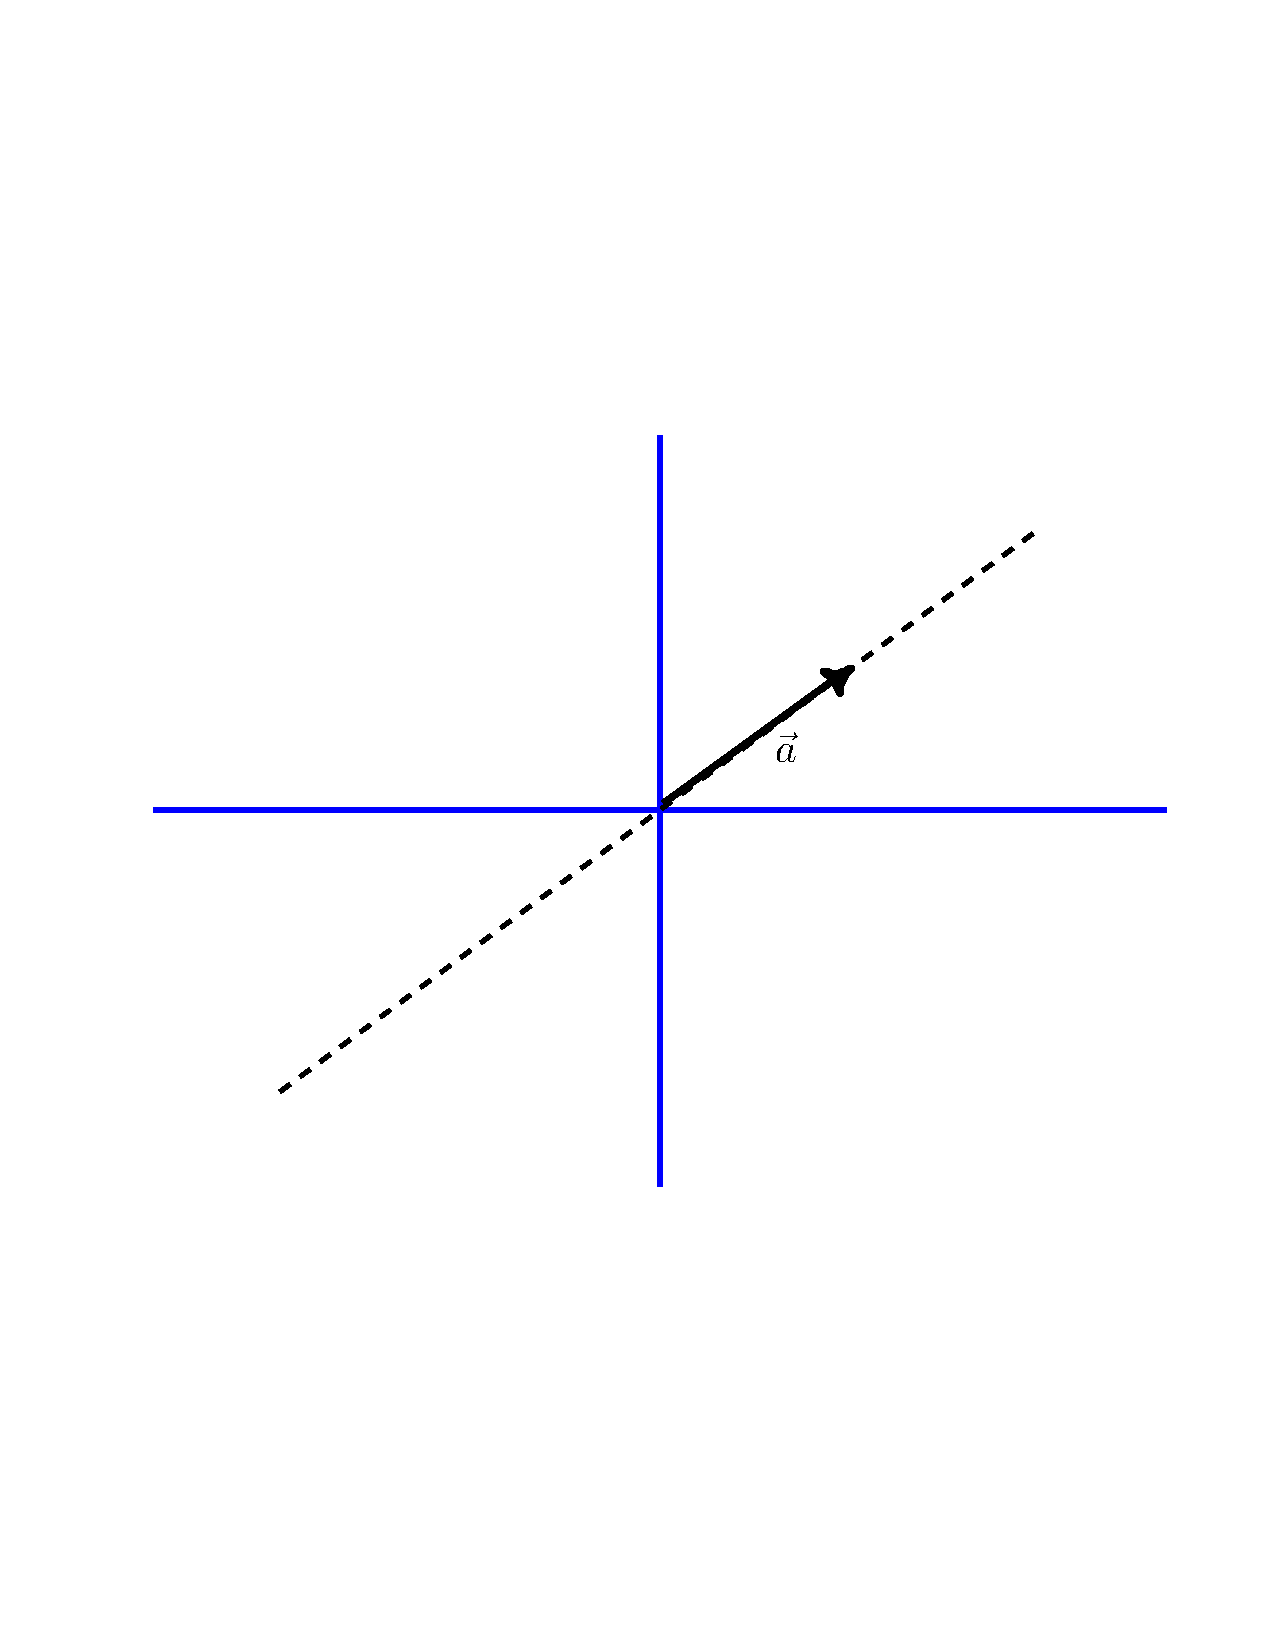
\includegraphics[height=3in]{2_2009_a1_3}}
\caption{Figure for Example \ref{2009_a1_3}. \label{ch2exnew1}}
\end{figure}

\subsection{Co-ordinates}

In order to do calculations with vectors, we have to introduce
co-ordinate axes.  Once we have chosen in what directions the
co-ordinate axes will lie, we can specify a vector by giving its
components in the co-ordinate directions.

\begin{figure}
\centerline{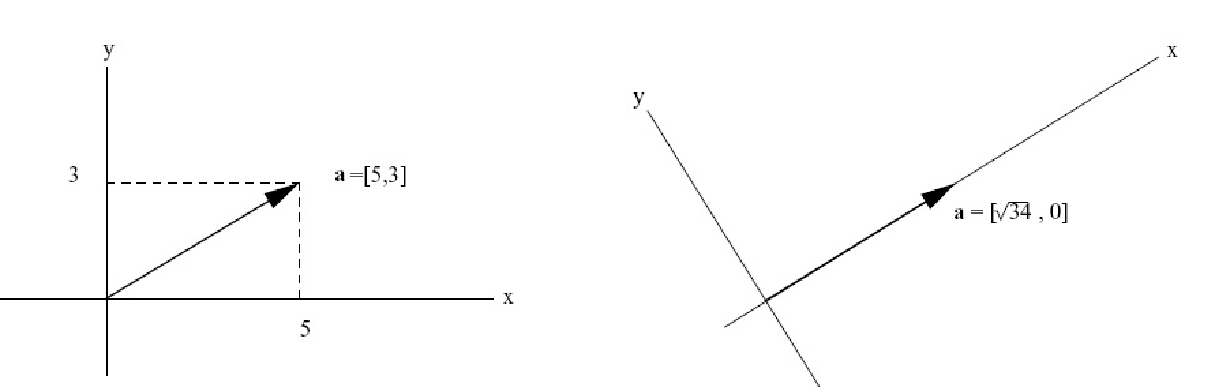
\includegraphics[height=2in]{2_coords}}
\caption{Two choices of co-ordinate axes. \label{fig_coords}}
\end{figure}

In the Figure~\ref{fig_coords} 
we see two choices of $x$ and $y$ axes. For the first
choice of axes, the vector $\aa$ has co-ordinates $[5,3]$ and for the
second choice of axes the co-ordinates are $[\sqrt{34},0]$. In a given
problem, it makes sense to choose the axes so that at least some of
the vectors have a simple representation. For example, in analyzing
the forces acting on a pendulum, we would either choose the $y$ axis
either to be vertical, or to lie along the shaft of the pendulum.

We can choose to write the co-ordinates of a vector in a row, as
above, or in a column, like
\[
\left[ \begin{array}{c} 
5 \\ 3 \end{array}
\right]
\]
Later on, we will almost always write vectors as columns. But in this
chapter we will write vectors as rows. Writing vectors as rows saves
space on the page but we will learn later how to write vectors in row
form even when we want them to be column vectors for other reasons. 
{\bf Note:} When writing vector coordinates by hand or in this text, either 
square or round brackets can be used. However, when using MATLAB, 
vectors must be created with square brackets (round brackets are used 
for other purposes). Other packages such as the online homework system, 
WeBWorK, may require different syntax. 

A convenient way to choose the co-ordinate axes is to specify unit
vectors (that is, vectors of length one) that lie along each of the
axes. These vectors are called standard basis vectors and are denoted
${\bf i}$ and ${\bf j}$ (in two dimensions) and ${\bf i}$, ${\bf j}$
and ${\bf k}$ (in three dimensions). These vectors are shown in 
Figure~\ref{fig_unitvecs}. Sometimes they are also denoted
${\bf e}_1$ and ${\bf e}_2$ or $\hat{\imath}$ and $\hat{\jmath}$ 
(in two dimensions) and ${\bf e}_1$, 
${\bf e}_2$ and ${\bf e}_3$ or $\hat{\imath}$, $\hat{\jmath}$ and $\hat{k}$ (in three dimensions). 
Different application areas have different conventions. 

\begin{figure}
\centerline{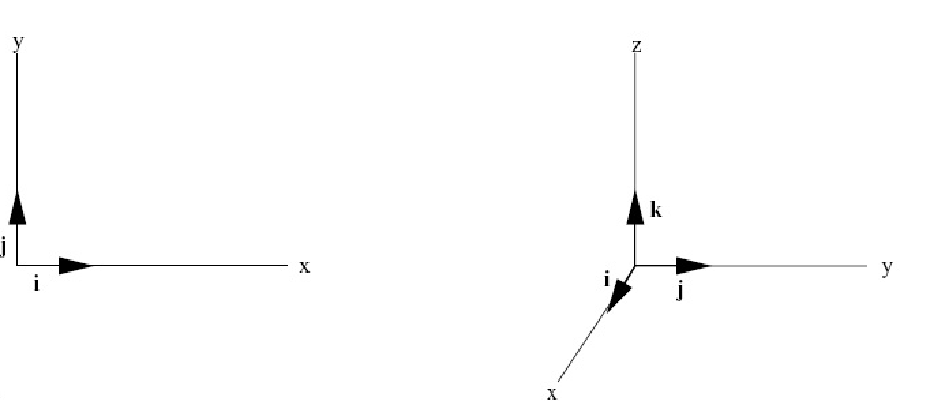
\includegraphics[height=2in]{2_unitvecs}}
\caption{Unit vectors in 2D (left) and 3D (right). \label{fig_unitvecs}}
\end{figure}

The unit vectors have co-ordinates 
\begin{eqnarray*}
{\bf i} &=& {\bf e}_1=[1,0] \\
{\bf j} &=& {\bf e}_2=[0,1] 
\end{eqnarray*}
in two dimensions, and
\begin{eqnarray*}
{\bf i}&=&{\bf e}_1=[1,0,0] \\
{\bf j}&=&{\bf e}_2=[0,1,0] \\
{\bf k}&=&{\bf e}_3=[0,0,1]
\end{eqnarray*}
in three dimensions.

Often, we make no distinction between a vector and its co-ordinate
representation. In other words, we regard the co-ordinate axes as
being fixed once and for all. Then a vector in two dimensions is
simply a list of two numbers (the components) $[a_1,a_2]$, and a
vector in three dimensions is a list of three numbers
$[a_1,a_2,a_3]$. Vectors in higher dimensions are now easy to
define. A vector in $n$ dimensions is a list of $n$ numbers
$[a_1,a_2,\ldots,a_n]$.

When a vector is multiplied by a number, each component is scaled by
the same amount. Thus if $\aa = [a_1,a_2]$, then
\begin{eqnarray*}
s\aa &=& s[a_1,a_2] \\
&=& [sa_1,sa_2]
\end{eqnarray*}

Similarly, when two vectors are added, their co-ordinates are added
component-wise. So if $\aa = [a_1,a_2]$ and $\bb=[b_1,b_2]$, then
\begin{eqnarray*}
\aa+\bb&=&[a_1,a_2]+[b_1,b_2]\\
&=&[a_1+b_1,a_2+b_2]
\end{eqnarray*}
This is shown in Figure~\ref{fig_coordadd}. 

\begin{figure}
\centerline{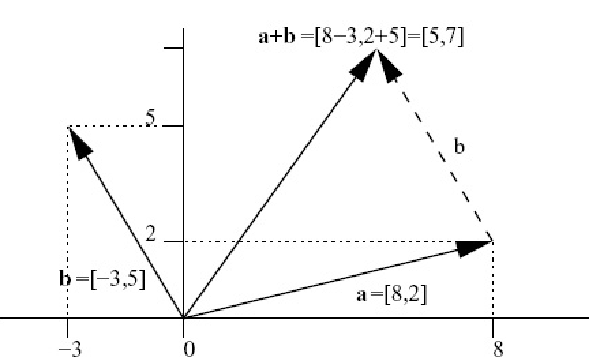
\includegraphics[height=2in]{2_coordadd}}
\caption{Adding vector co-ordinates. \label{fig_coordadd}}
\end{figure}

The analogous formulae hold in three (and higher dimensions). If 
$\aa=[a_1,a_2,\ldots,a_n]$ and $\bb = [b_1,b_2,\ldots,b_n]$, then
\begin{eqnarray*}
s\aa &=& s[a_1,a_2,\ldots,a_n]\\
&=&[sa_1,sa_2,\ldots,sa_n]\\
\aa+\bb&=&[a_1,a_2,\ldots,a_n]+[b_1,b_2,\ldots,b_n]\\
&=&[a_1+b_1,a_2+b_2,\ldots,a_n+b_n]
\end{eqnarray*}

\begin{example}
\label{2008_a1_1}
Sketch axes $x_1$-$x_2$. Add the vectors (1,1) and (2,-1) to
your sketch. Draw these vectors with base point at the origin. Now add
the vector (1,-2) to your sketch, starting at the base point
(1,1). That is, draw the vector with components 1 to the right and 2
down starting at (1,1). {\bf Note:}\ your sketch should show
graphically that (1,1)+(1,-2)=(2,-1). {\rm See Figure~\ref{ch2exnew2}.}
\end{example}

\begin{figure}[htb]
\centerline{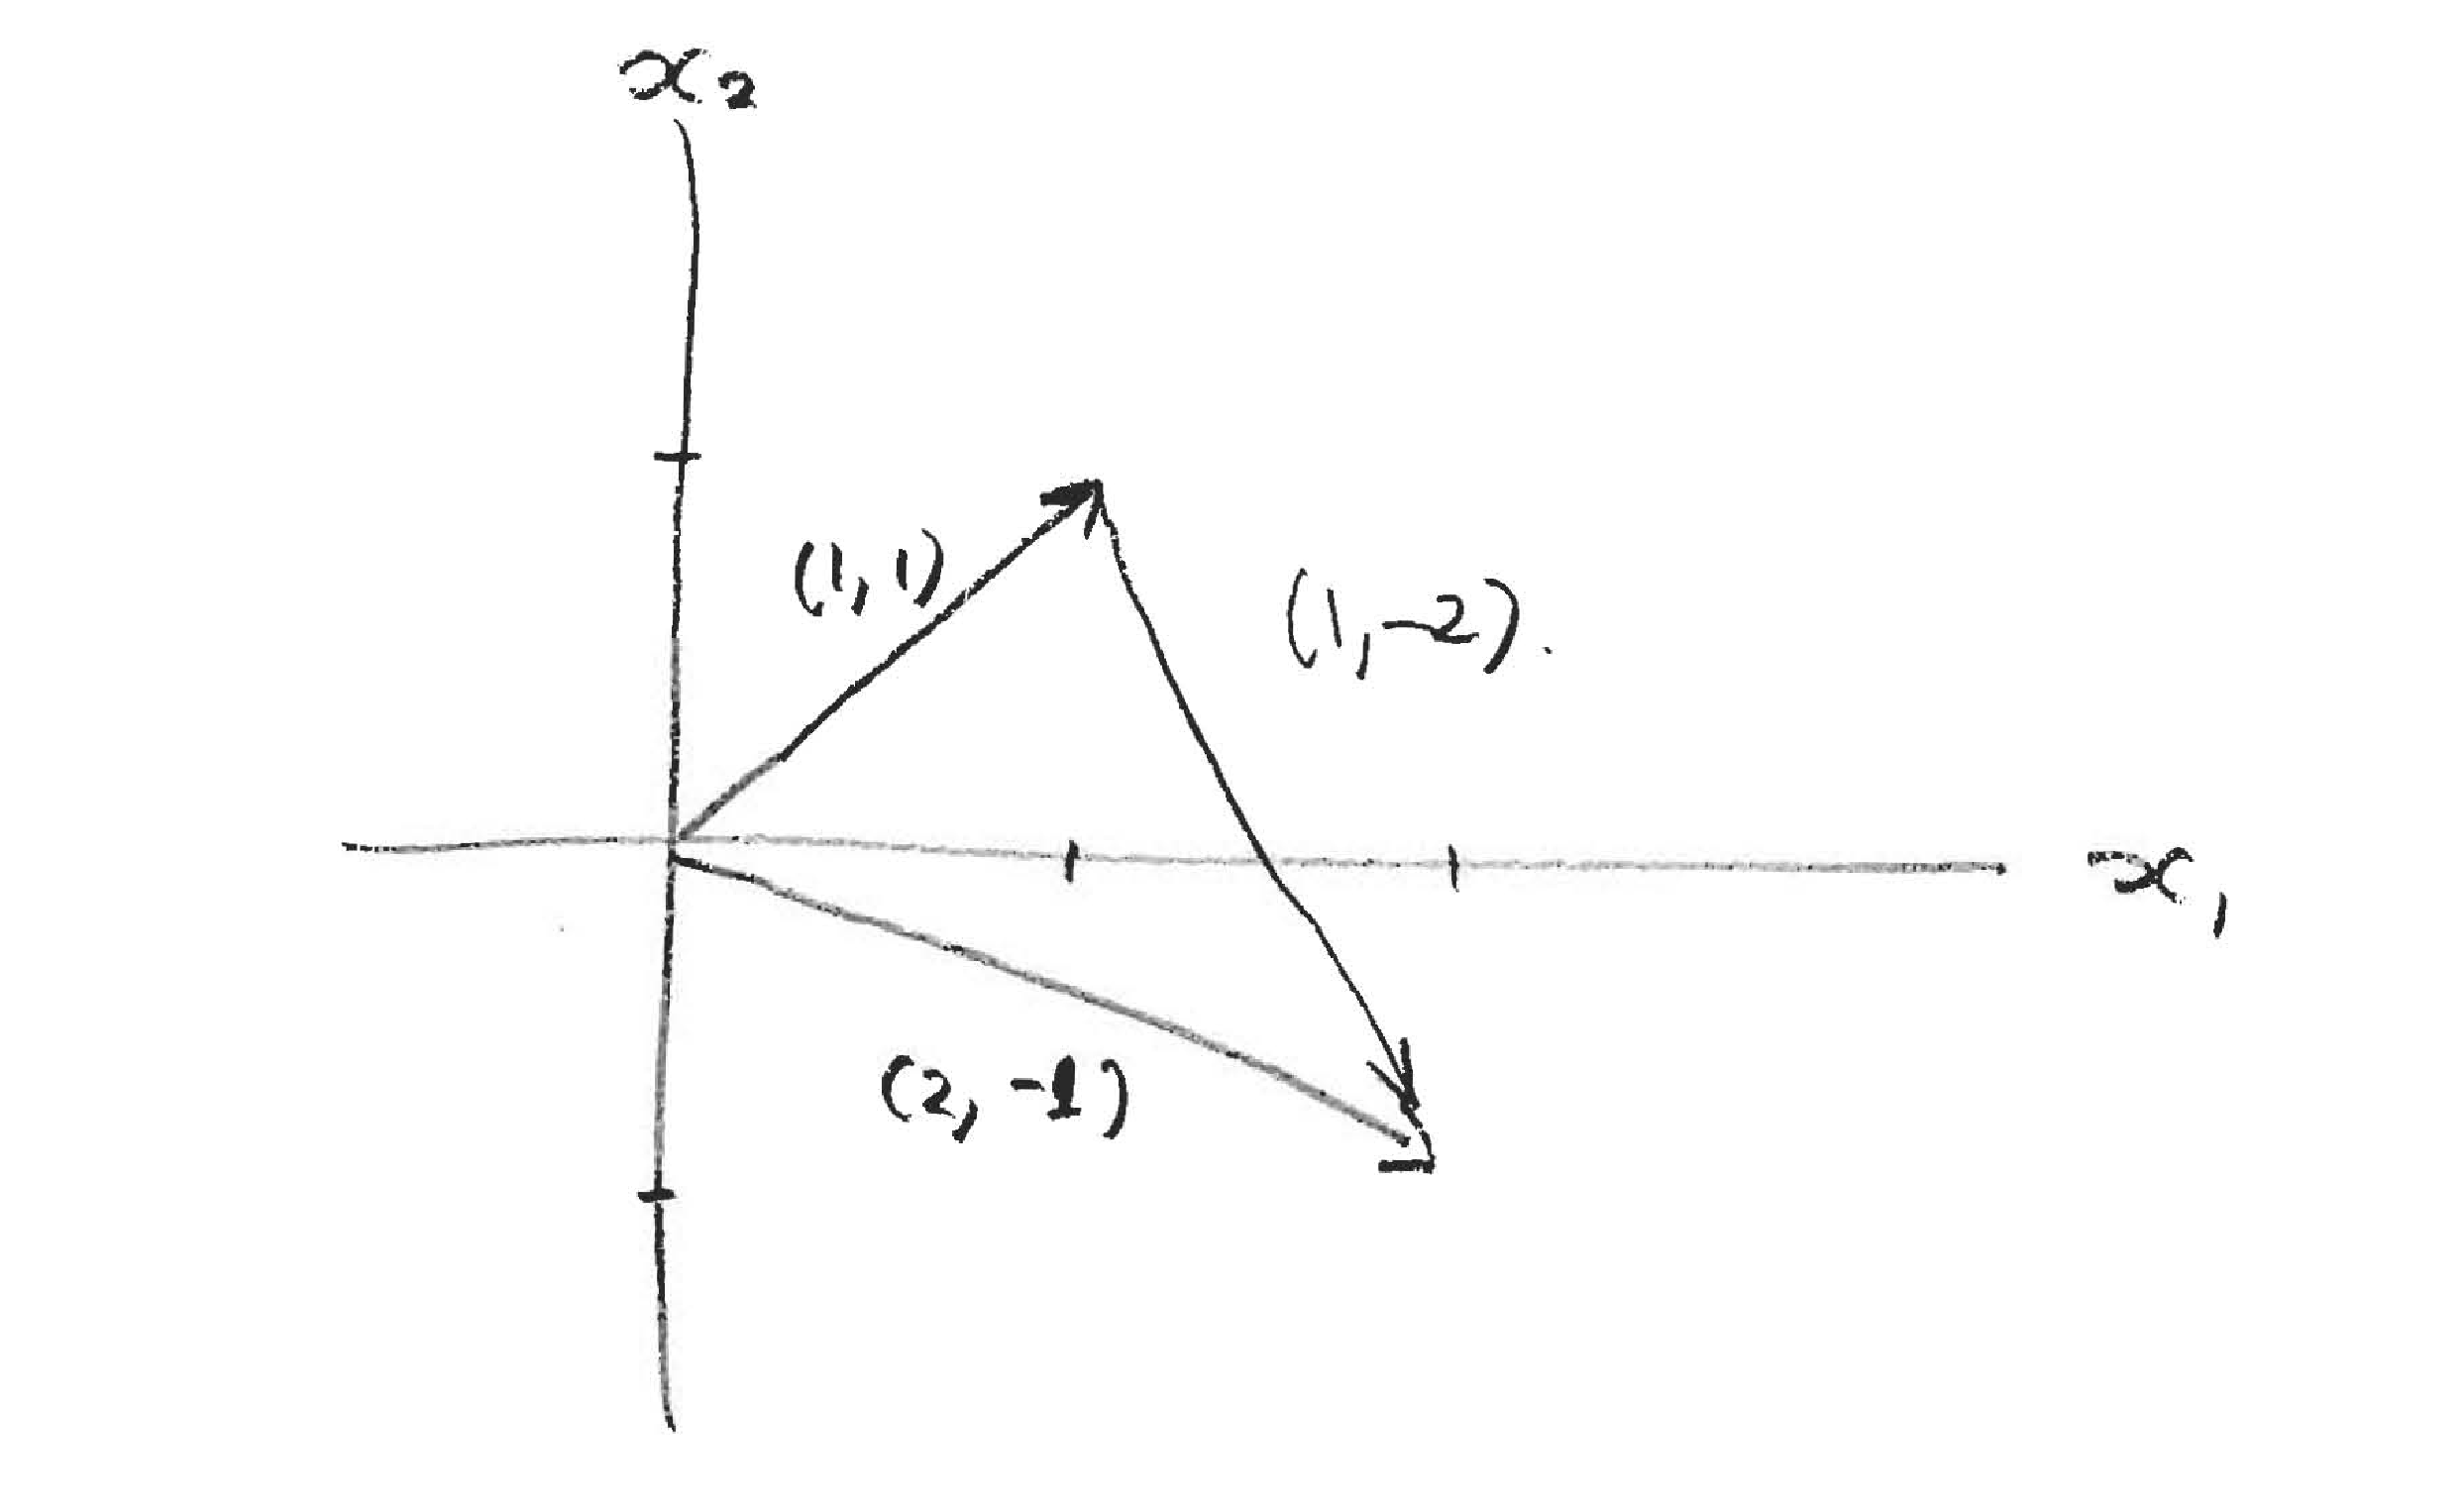
\includegraphics[height=1.5in]{2_newfig1}}
\caption{Figure for example \ref{2008_a1_1} \label{ch2exnew2}}
\end{figure}

\subsection{Properties of vector addition and scalar multiplication}

Let $\zv$ denote the zero vector. This is the vector all of whose
components are zero. The following properties are intuitive and easy
to verify.

\begin{enumerate}
\item $\aa+\bb=\bb+\aa$	
\item $\aa+(\bb+\cc)=(\aa+\bb)+\cc$
\item $\aa+\zv=\aa$
\item $\aa+(-\aa)= \zv$
\item $s(\aa+\bb)=(s\aa+s\bb)$
\item $(s+t)\aa=s\aa+t\aa$
\item $(st)\aa=s(t\aa)$	
\item $1\aa=\aa$
\end{enumerate}

They follow from similar properties which hold for numbers. For
example, for numbers $a_1$ and $b_1$ we know that $a_1+b_1 =
b_1+a_1$. Thus
\begin{eqnarray*}
\aa + \bb & = & [a_1,a_2]+[b_1,b_2] \\
& = & [a_1+b_1,a_2+b_2] = [b_1+a_1,b_2+a_2] \\
& = & [b_1,b_2]+[a_1,a_2] = \bb+ \aa, \\
\end{eqnarray*}
so property 1 holds.  Convince yourself that the rest of these
properties are true. (What is the vector $-\aa$?). It might seem like
a waste of time fussing over obvious properties such as
these. However, we will see when we come to the cross product and
matrix product, that sometimes such ``obvious'' properties turn out to
be false! It is important to know what the allowable operations for vectors 
(and matrices which we will see in later chapters) are since we will be doing 
algebra to solve matrix and vector equations. We will take special care to 
highlight the operations that have different properties from the scalar case.  

\subsection{MATLAB: basic scalar and vector operations}

There are MATLAB computer labs that accompany this course at UBC. You will be given 
an account on the Mathematics Department undergraduate network and instructions 
on how to access the computers in the labs and start the MATLAB application. 
A freely available google application, Octave, can execute all of the commands in the course 
with the same syntax. 
In the command window at the prompt {\tt >>} (MATLAB) or $\rhd$ (Octave), 
you can type MATLAB commands directly. Some basic commands are given below 
\begin{description}
\item[{\bf assignment:}] Scalar and vector variables can be assigned 
using the ``=" operator. For example 
\begin{verbatim}
a = 2 
\end{verbatim}
followed by {\tt <enter>} 
assigns the scalar value of 2 to the variable {\tt a}. The result 
of the command is printed out although this can be suppressed by using a 
colon at the end of the command:
\begin{verbatim}
a = 2;
\end{verbatim}
Here {\tt a} is still assigned the value of 2 but no output is generated. 
Vector variables are assigned with the following notation:
\begin{verbatim}
b = [1 2];
\end{verbatim}
Note that {\tt b = [1, 2]} has the same meaning in MATLAB, i.e., numbers separated by a comma or a space imply row vectors. For column vectors, the entries have to be separated by semicolons:
\begin{verbatim}
b1 = [2; 3];
\end{verbatim}

Note also that there are no special distinctions between the names of scalar and
vector variables. 
\item[{\bf addition:}] Both scalar and vector addition can be done with 
the ``+" operator. Keeping the values of scalar {\tt a} and vector {\tt b} 
above, we enter the commands
\begin{verbatim}
a2 = 5;
b2 = [2 9];
a+a2
c = b+b2;
\end{verbatim}
The first two lines above assign a new scalar and vector. The third line 
prints out the answer 7 (2+5). The last line assigns the resulting vector 
[3 11] ([1 2] + [2 9]) to the new vector {\tt c} but prints nothing. 
\item[{\bf scalar multiplication}] Scalar multiplication (of vectors and 
other scalars) is implemented using the ``*" command. Using the variables 
defined above,
\begin{verbatim}
a*a2
a*b 
\end{verbatim}
would result in 10 (2 times 5) and [2 4] (2 times [1 2]). The ``*" command 
also implements matrix-vector and matrix-matrix multiplication discussed 
later in the course. Vector-vector multiplication (dot products and 
cross products) are implemented using different commands as discussed in the 
next section. 
\item[{\bf other commands:}] There are many useful functions built 
in to MATLAB such as {\tt sqrt} (square root), {\tt cos} (cosine, taking 
an argument in radians), {\tt acos} (inverse cosine, giving an result 
in radians) and many more. They are called as follows
\begin{verbatim}
sqrt(2)
\end{verbatim}
which will return $\sqrt{2}$ to 4 decimal places. Type {\tt help} followed
by a command name gives you a description of that command. Try 
typing {\tt help atan2} since {\tt atan2} is a pretty useful function. 
These MATLAB functions can take vector arguments, they act on each 
entry of the vector. For example 
\begin{verbatim}
sqrt([1 4])
\end{verbatim}
will produce the vector [1 2]. 
\end{description}

\subsection{Problems} 

\begin{problem}
  \label{2009_a1_1}
Sketch axes $x_1$-$x_2$. Add the vectors (2,2) and (1,-1) to
your sketch. Draw these vectors with base point at the origin. Now add
the vector (1,-1) to your sketch, starting at the base point
(2,2). That is, draw the vector with components 1 to the right and 1
down starting at (2,2). {\bf Note:}\ your sketch should show
graphically that (2,2)+(1,-1)=(3,1).
\end{problem}

\begin{problem}
\label{op1_1}
Let $\aa$, $\bb$ and $\cc$ be fixed non-zero vectors. Describe and
sketch the following sets of points in two and three dimensions:
\begin{enumerate}
\renewcommand{\labelenumi}{(\roman{enumi})}
\item $\{s\aa : s\in\RR\}$ (i.e., the set of all scalar multiples of
$\aa$)\par
\item $\{s\aa : s>0\}$ (i.e., the set of all positive scalar multiples
of $\aa$)\par
\item $\{\bb + s\aa : s\in\RR\}$\par
\item $\{s\aa + t\bb : s,t\in\RR\}$\par
\item $\{\cc + s\aa + t\bb : s,t\in\RR\}$\par
\end{enumerate}
\end{problem}

\begin{problem}
\label{op1_2}
Describe the vectors $\aa - \bb$ and $\bb - \aa$.
\end{problem}

\begin{problem}
\label{op1_3}
Find an expression for the midpoint between $\aa$ and $\bb$. Find an expression
for a point one third of the way between $\aa$ and $\bb$.
\end{problem}

\begin{problem}
\label{op1_4}
Find an expression for the line segment joining $\aa$ and $\bb$.
\end{problem}

\section{Geometrical Aspects of Vectors}

\subsection{Length of a vector}

It follows from the Pythagorean formula that the length $\|\aa\|$ of
$\aa=[a_1,a_2]$ satisfies $\|\aa\|^2=a_1^2+a_2^2$. This is shown in 
Figure~\ref{fig_pyth}.

\begin{figure}
\centerline{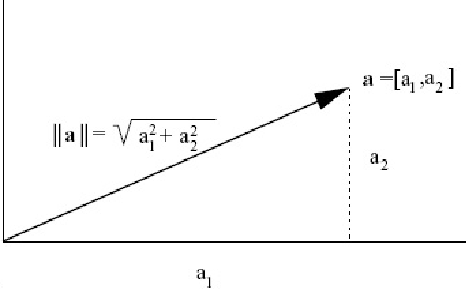
\includegraphics[height=2in]{2_pyth}}
\caption{Pythagorean Formula. \label{fig_pyth}}
\end{figure}

Thus
\[
\|\aa\|= \sqrt{a_1^2+a_2^2}.
\]
Similarly, for a vector $\aa=[a_1,a_2,a_3]$ in three dimensions,
\[
\|\aa\|= \sqrt{a_1^2+a_2^2+a_3^2}.
\]
The distance between two vectors $\aa$ and $\bb$ is the length of the
difference $\bb-\aa$.

\subsection{The dot product}

The dot product of two vectors is defined in both two and three
dimensions (actually in any dimension). The result is a number. Two
main uses of the dot product are testing for orthogonality and
computing projections.

The dot product of $\aa=[a_1,a_2]$ and $\bb=[b_1,b_2]$ is given by
\[
\aa\cdot\bb = a_1b_1 + a_2b_2.
\]
Similarly, the dot product of $\aa=[a_1,a_2,a_3]$ and
$\bb=[b_1,b_2,b_3]$ is given by
\[
\aa\cdot\bb = a_1b_1 + a_2b_2 + a_3b_3.
\]
The properties of the dot product are as follows:
\begin{description}
\item[0.] If $\aa$ and $\bb$ are vectors, then $\aa\cdot\bb$ is a number.
\item[1.] $\aa\cdot\aa = \|a\|^2$.
\item[2.] $\aa\cdot\bb = \bb\cdot\aa$.
\item[3.] $\aa\cdot(\bb+\cc) = \aa\cdot\bb + \aa\cdot\cc$.
\item[4.] $s(\aa\cdot\bb) = (s\aa)\cdot\bb$.
\item[5.] $\zv\cdot\aa=0$.
\item[6.] $\aa\cdot\bb = \|\aa\|\|\bb\|\cos(\theta)$, where $\theta$
is angle between $\aa$ and $\bb$.  
\item[7.] $\aa\cdot\bb = 0$ $\iff$ $\aa=\zv$ or $\bb=\zv$ or $\aa$ and
$\bb$ are orthogonal (i.e,. perpendicular).
\end{description}
Properties 0 to 5 are easy consequences of the definitions. 
For example, to
verify property 5 we write
\[
\zv\cdot\aa = [0,0,0]\cdot[a_1,a_2,a_3]= 0a_1+0a_2+0a_3=0.
\]

Property 6 is the most important property and is often taken as the
definition of the angle $\theta$ between vectors $\bf a$ and $\bf b$.  
Notice that our definition is given in terms of the
components of the vectors, which depend on how we chose the
co-ordinate axes. It is not at all clear that if we change the
co-ordinate axis, and hence the co-ordinates of the vectors, that we
will get the same answer for the dot product. However, property 6 says
that the dot product only depends on the lengths of the vectors and
the angle between them. These quantities are independent of how
co-ordinate axes are chosen, and hence so is the dot product.

To show that property 6 holds we compute $\|\aa-\bb\|^2$ in two
different ways.  First of all, using properties 1 to 5, we have
\begin{eqnarray}
\nonumber
\|\aa-\bb\|^2 & = & (\aa-\bb)\cdot(\aa-\bb) \\
 \nonumber
 & = & \aa\cdot\aa - \aa\cdot\bb - \bb\cdot\aa + \bb\cdot\bb \\
\label{ch2_theta1}
 & = & \|\aa\|^2 + \|\bb\|^2 - 2 \aa\cdot\bb
\end{eqnarray}
(Which properties were used in each step?) Next we compute
$\|\aa-\bb\|$ as depicted in Figure~\ref{fig_cos2} (left). 

\begin{figure}
\centerline{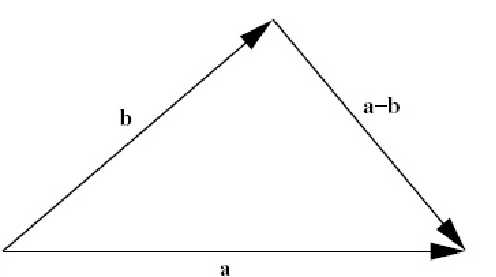
\includegraphics[height=1.5in]{2_cos1}
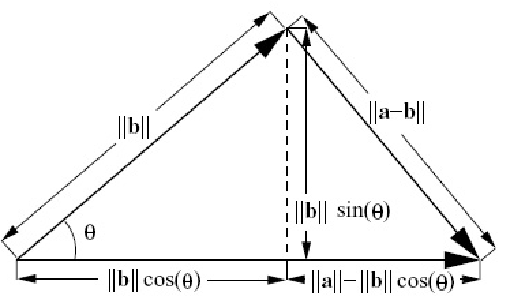
\includegraphics[height=1.5in]{2_cos2}}
\caption{The vectors $\aa$, $\bb$ and $\aa-\bb$ (left) 
Lengths of Segments (right). \label{fig_cos2}}
\end{figure}

We mark the lengths of each of the line segments in Figure~\ref{fig_cos2}
(right). 
Using Pythagoras' theorem for the right angled triangle on the right
of this diagram, we see that
\[
\|\aa-\bb\|^2 = (\|\aa\|-\|\bb\|\cos(\theta))^2 + \|\bb\|^2\sin^2(\theta).
\]
Thus, using $\cos^2(\theta)+\sin^2(\theta)=1$,
\begin{eqnarray}
\nonumber
\|\aa-\bb\|^2 & = & \|\aa\|^2+\|\bb\|^2\cos^2(\theta) -
2\|\aa\|\|\bb\|\cos(\theta) + \|\bb\|^2\sin^2(\theta) \\
\label{ch2_theta2}
 & = & \|\aa\|^2+\|\bb\|^2 - 2\|\aa\|\|\bb\|\cos(\theta)
\end{eqnarray}
Actually, this is just the cosine law applied to the triangle in Figure~\ref{fig_cos2}
and you may have been able to write (\ref{ch2_theta2}) directly. 
Now we equate the two expressions (\ref{ch2_theta1}, \ref{ch2_theta2}) 
for $\|\aa-\bb\|^2$. This gives
\[
\|\aa\|^2 + \|\bb\|^2 - 2 \aa\cdot\bb = \|\aa\|^2+\|\bb\|^2 -
2\|\aa\|\|\bb\|\cos(\theta)
\]
Subtracting $\|\aa\|^2 + \|\bb\|^2$ from both sides and dividing by
$-2$ now yields
\[
\aa\cdot\bb=\|\aa\|\|\bb\|\cos(\theta).
\]
This proves property 6.

Property 7 now follows directly from 6. If $\aa\cdot\bb = 0$ then
$\|\aa\|\|\bb\|\cos(\theta)=0$ so either $\|\aa\|=0$, in which case
$\aa=\zv$, or $\|\bb\|=0$, in which case $\bb=\zv$, or
$\cos(\theta)=0$, which implies that $\theta = \pi/2$ (since $\theta$
lies between $0$ and $\pi$).  This implies $\aa$ and $\bb$ are
orthogonal.

Property 6 can be used to compute the angle between two vectors as shown in the example below.  
\begin{example}
What is the angle between the vectors whose tails lie at the
centre of a cube and whose heads lie on adjacent vertices?  {\rm To compute
this take a cube of side length $2$ and centre it at the origin, so
that the vertices lie at the points $[\pm 1, \pm 1, \pm1]$.  Then we
must find the angle between $\aa=[1, 1, 1]$ and $\bb=[-1, 1, 1]$.
Since
\[
\aa\cdot\bb = -1 + 1 + 1 = 1 =
\|\aa\|\|\bb\|\cos(\theta)=\sqrt{3}\sqrt{3}\cos(\theta)
\]
we obtain
\[
\theta = \arccos(1/3) \sim 1.231 \quad (\sim 70.5^\circ)
\]}
\end{example}

\begin{example}
For what value (or values) of $s$ is the vector $[1,1,s]$ perpendicular to  $[1,5,3]$? 
{\rm The dot product of the two vectors must be zero for them to be orthogonal. We compute 
\[
[1,1,s] \cdot [1,5,3] = 1+5+3s 
\]
so $6+3s=0$ for orthogonality, $s=-2$.} 
\end{example} 

Here is an example to review the basic operations on vectors we know so far.
\begin{example}
% \label{2008_a1_2}
Consider the vectors ${\bf a} = (2,3)$ and ${\bf b} =
(1,-3)$ in $\mathbb{R}^2$. Compute the following:
{\begin{enumerate}
\renewcommand{\labelenumi}{(\alph{enumi})}
\item ${\bf a} + {\bf b}$
\item $3 {\bf a}$
\item $2{\bf a} + 4{\bf b}$
\item ${\bf a} \cdot {\bf b}$
\item $\| {\bf b} \|$
\end{enumerate}}
{\rm Solutions:
\begin{enumerate}
\renewcommand{\labelenumi}{(\alph{enumi})}
\item $\aa + \bb = (2,3)+(1,-3) = (3,0)$
\item $3 \aa = 3 (2,3) = (6,9)$
\item $2\aa + 4\bb = 2(2,3) + 4(-1,3) = (4,6)+(4,-12) = (8,-6)$
\item $\aa \cdot \bb = (2,3) \cdot (1,-3) = 2-9 = -7$.
\item $\| \bb \| = \sqrt{1^2 + (-3)^2} = \sqrt{10}$.
\end{enumerate}}
\end{example}

\subsection{Projections and Unit Vectors}

Suppose $\aa$ and $\bb$ are two vectors. The projection of $\aa$ in
the direction of $\bb$, denoted ${\rm proj}_\bb\aa$, is the vector in
the direction of $\bb$ whose length is determined by drawing a line
perpendicular to $\bb$ that goes through $\aa$.  In other words, the
length of ${\rm proj}_\bb\aa$ is the component of $\aa$ in the
direction of $\bb$. This is shown in Figure~\ref{fig_proj}

\begin{figure}
\centerline{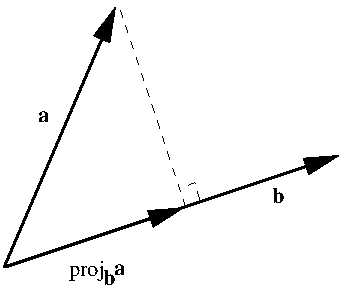
\includegraphics[height=1.5in]{2_proj}}
\caption{Projection. \label{fig_proj}}
\end{figure}

To compute ${\rm proj}_\bb\aa$, we first note that it is a multiple of
$\bb$.  Thus ${\rm proj}_\bb\aa = s\bb$ for some number $s$. To
compute $s$, we use the fact that the vector ${\rm proj}_\bb\aa - \aa$
(along the dotted line in the diagram) is orthogonal to $\bb$. Thus
$({\rm proj}_\bb\aa - \aa)\cdot\bb = 0$, or $(s\bb-\aa)\cdot\bb=0$, or
$s = \aa\cdot\bb / \bb\cdot\bb = \aa\cdot\bb / \|\bb\|^2$. Thus
\begin{equation}
\label{eq:projection}
{\rm proj}_\bb\aa = {{\aa\cdot\bb}\over{\|\bb\|^2}}\bb.
\end{equation}
If $\bb$ is a unit vector (i.e., $\|\bb\|=1$, length 1) this expression is even
simpler. We will use the notation $\hat{b}$ to denote unit vectors. In this case
\[
{\rm proj}_{\hat{b}} \aa = (\aa\cdot\hat{b})\,\hat{b}.
\]

It is easy to find a unit vector $\hat{b}$ that points in the same direction as any nonzero 
vector $\bb$, simply compute 
\[
\hat{b} = \frac{1}{\| \bb \|} \bb.
\]
Since $\hat{b}$ is a (positive) scalar multiple of $\bb$ in the above formula, it clearly points in the
same direction as $\bb$. A straight forward calculation shows that $\hat{b}$ has unit length 
(try it!). 

\begin{example}
Find the unit vector $\hat{b}$ that points in the same direction as $\bb = [1, 2]$.
{\rm We compute 
\[
\| \bb \| = \sqrt{1^2 + 2^2} = \sqrt{5}
\]
and then 
\[
\hat{b} = \frac{1}{\sqrt{5}} [1,2] = [1/\sqrt{5}, 2/\sqrt{5}]. 
\]} 
\end{example}

Projections are useful for computing the components of a vector in
various directions. An easy example is given be the co-ordinates of a
vector. These are simply the components of a vector in the direction
of the standard basis vectors. So in two dimensions
\begin{eqnarray*}
a_1 & = & \aa\cdot{\bf i} = [a_1,a_2]\cdot[1,0] \\
a_2 & = & \aa\cdot{\bf j} = [a_1,a_2]\cdot[0,1]
\end{eqnarray*}

\begin{example}
Let $\aa = [1,0,2]$ and $\bb = [0, 5, 2]$. Compute 
$ \mbox{proj}_{\bf b} {\bf a}$ (the projection of $\bf a$ in the
direction of $\bf b$).
{\rm We use (\ref{eq:projection}) and first compute 
\[
\| \bb \|^2 = 5^2 + 2^2 = 29 \mbox{\ \ \ and $\aa \cdot \bb = 4$}, 
\]
then 
\[
\mbox{proj}_{\bf b} {\bf a} = \frac{4}{29} [0, 5, 2] = [0, 20/29, 8/29].
\]}
\end{example}

\subsection{MATLAB: {\tt norm} and {\tt dot}  commands}

MATLAB has built-in functions that implement most of the mathematical 
operations introduced this course. For example, the commands 
\begin{description}
\item[{\tt norm(a)}] returns the length (norm) of the vector {\tt a}. 
\item[{\tt dot(a,b)}] returns the dot product of the vectors 
{\tt a} and {\tt b} (if the vectors do not have the same length, an 
error results as you would expect). 
\end{description}
Using these commands and scalar multiplication of vectors, a projection 
of {\tt a} onto the direction {\tt b} can be implemented:
\begin{verbatim}
(dot(a,b)/norm(b)^2))*b
\end{verbatim}
where {\tt /} denotes division (of scalar quantities in this case) and 
{\tt \^\ p} gives the p'th power of a quantity. 

\subsection{Problems}

\begin{problem}
  \label{2009_a1_2}
Consider the vectors ${\bf a} = (1,2)$ and ${\bf b} =
(1,-2)$ in $\mathbb{R}^2$ (the set of vectors with 2 components).
Compute the following:
\begin{enumerate}
\item ${\bf a} + {\bf b}$
\item $2 {\bf a}$
\item ${\bf a} - {\bf b}$
\item ${\bf a} \cdot {\bf b}$
\item $\| {\bf b} \|$
\end{enumerate}
\end{problem}

\begin{problem}
\label{2008_a1_3}
A circle in the $x_1$-$x_2$ plane has centre at (2,5). A given
point on its circumference is (3,3). Write an equation that describes
all the points $(x_1,x_2)$ on the circle. 
\end{problem}

\begin{problem}
\label{op1_5}
Find the equation of a sphere centred at $\aa=[a_1,a_2,a_3]$ with
radius $r$.  (Hint: the sphere is the set of points
$\xx=[x_1,x_2,x_3]$ whose distance from $\aa$ is $r$
\end{problem}

\begin{problem}
\label{op1_6}
Find the equation of a sphere if one of its diameters has endpoints
$[2,1,4]$ and $[4,3,10]$
\end{problem}

\begin{problem}
\label{op1_7}
Compute the dot product of the vectors $\aa$ and $\bb$ and find the angle
between them.
{\begin{enumerate}
\renewcommand{\labelenumi}{(\roman{enumi})}
\item $\aa=[1,2]$, $\bb=[-2,3]$
\item $\aa=[-1,2]$, $\bb=[1,1]$
\item $\aa=[1,1]$, $\bb=[2,2]$
\item $\aa=[1,2,1]$, $\bb=[-1,1,1]$
\item $\aa=[-1,2,3]$, $\bb=[3,0,1]$
\end{enumerate}}
\end{problem}

\begin{problem}
\label{2009_a1_4}
Let ${\bf a} = (1,1,1)$ and ${\bf b} = (3,1,-2)$. Compute the
following:
\begin{enumerate}
\item The angle between ${\bf a}$ and ${\bf b}$.
\item $ \mbox{proj}_{\bf a} {\bf b}$ (the projection of $\bf b$ in the
direction of $\bf a$).
\end{enumerate}
\end{problem}

\begin{problem}
\label{2008_a1_5}
Let ${\bf a} = (1,4,0)$ and ${\bf b} = (2,-1,5)$. Compute the
following:
{\begin{enumerate}
\renewcommand{\labelenumi}{(\alph{enumi})}
\item The angle between ${\bf a}$ and ${\bf b}$.
\item $ \mbox{proj}_{\bf a} {\bf b}$ (the projection of $\bf b$ in the
direction of $\bf a$). 
\end{enumerate}}
\end{problem}

\begin{problem}
\label{op1_8}
For which value of $s$ is the vector $[1,2,s]$ orthogonal to
$[-1,1,1]$?
\end{problem}

\begin{problem}
\label{op1_9}
Does the triangle with vertices $[1,2,3]$, $[4,0,5]$ and $[3,4,6]$
have a right angle? 
\end{problem}

\begin{problem}
\label{2009_a1_5}
Determine the values of $c_1$ and $c_2$ such that the vector
[$c_1$ 1 $c_2$] is a scalar multiple of [2 -2 3]. 
\end{problem}

\begin{problem}
\label{op1_10}
An air-plane with an approach speed of 70 knots is on approach to
runway 26 (i.e., pointing in the direction of 260 degrees). This 
is shown in Figure~\ref{fig_runway} (left). If the
wind is from 330 degrees at 10 knots, what heading should the pilot
maintain to stay lined up with the runway? What is the groundspeed of
the air-plane?
\end{problem}

\begin{figure}
\centerline{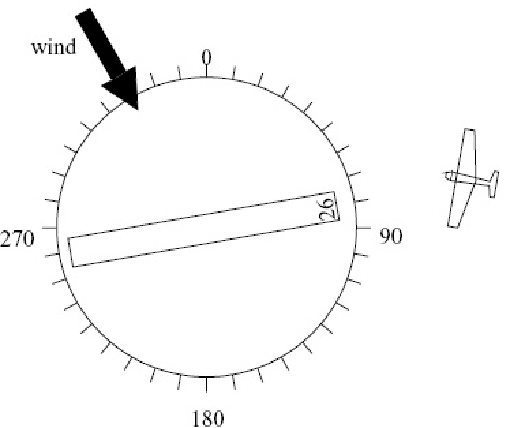
\includegraphics[height=1.5in]{2_runway}
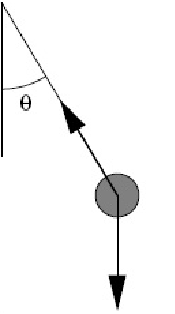
\includegraphics[height=1.5in]{2_pend2}}
\caption{Runway diagram for problem~\ref{op1_10} (left) and 
the pendulum of problem~\ref{op1_11} (right) \label{fig_runway}}
\end{figure}

\begin{problem}
\label{op1_11}
Suppose the angle of the pendulum shaft makes an angle of $\theta$
with the vertical direction as 
shown in Figure~\ref{fig_runway} (right). The force of gravity has
magnitude (length) equal to $mg$ and points downwards. The force along
the shaft of the pendulum acts to keep the shaft rigid, i.e., the
component of the total force along the shaft is zero. Write down the
co-ordinates of the two forces and the total force using two different
sets of co-ordinate axes --- one horizontal and vertical, and one
parallel to and orthogonal to the shaft of the pendulum.
\end{problem}


\begin{problem}
\label{matlab_op1_11}
(Matlab) In Matlab code, if one defines a vector $\aa=[a_1,a_2,\cdots,a_n]$, with the $a_i$'s being any numbers, the output of typing $\aa(j)$ would be $a_j$.

Suppose that you have a two element vector. How would you write a line of Matlab code to compute the norm of the vector, without using the {\tt norm} or {\tt dot} commands?
\end{problem}

\section{Determinants and the Cross Product}

\subsection{The determinant in two and three dimensions}
\label{s:trick} 

The determinant is a number that is associated with a square matrix,
that is, a square array of numbers.

In two dimensions it is defined by
\[
\det\left[\matrix{a_1&a_2\cr b_1&b_2\cr}\right]=a_1b_2-a_2b_1.
\]

\begin{example}
Find the determinant of 
\[
\left[\matrix{1 & 2 \cr 3 & 4 \cr}\right].
\]
{\rm Using the formula above, we have that the determinant is 
\[
1\times 4 - 2 \times 3 = -2. 
\]
}
\end{example}

\noindent The definition in three dimensions is
\begin{eqnarray*}
\det \left[ \begin{array}{ccc}
	a_1&a_2&a_3 \\
	b_1&b_2&b_3 \\
	c_1&c_2&c_3
	    \end{array}
\right]
 & = & a_1\det\left[\matrix{b_2&b_3\cr c_2&c_3\cr}\right]
       - a_2\det\left[\matrix{b_1&b_3\cr c_1&c_3\cr}\right]
+ a_3\det\left[\matrix{b_1&b_2\cr c_1&c_2\cr}\right] \\
 & = & a_1b_2c_3-a_1b_3c_2 + a_2b_3c_1-a_2b_1c_3 + a_3b_1c_2-a_3b_2c_1
\end{eqnarray*}

We want to determine the relationship between the determinant and the
vectors $\aa=[a_1,a_2]$ and $\bb = [b_1,b_2]$ (in two dimensions) and
$\aa=[a_1,a_2,a_3]$, $\bb = [b_1,b_2,b_3]$ and $\cc=[c_1,c_2,c_3]$ (in
three dimensions). We will do the two dimensional case now, but
postpone the three dimensional case until after we have discussed the
cross product.

\begin{example}
Find the determinant of 
\[
A = \left[ \begin{array}{ccc}
	1 & 1 & 0 \\
	4 & 2 & 2 \\
	1 & 0 & 3
	    \end{array}
\right].	    
\]
{\rm It is easiest to remember the formula using the first line in the equation above 
using the determinants of the corresponding $2 \times 2$ blocks of the matrix. 
\[
\det A = 1 (2 \times 3-0) -1 (4 \times 3 -2) + 0 = -4. 
\]
}
\end{example}

So let $\aa=[a_1,a_2]$ and $\bb = [b_1,b_2]$ be two vectors in
the plane. Define
\[
\aa^\perp = [-a_2,a_1].
\]
Notice that $\aa^\perp$ has the same length as $\aa$, and is
perpendicular to $\aa$, since
\[
\aa^\perp\cdot\aa = -a_2a_1 + a_1a_2 = 0.
\]
There are exactly two vectors with these properties. The vector
$\aa^\perp$ is the one that is obtained from $\aa$ by a counterclockwise
rotation of $\pi/2$ (i.e., $90^\circ$). To see this, notice that if
$\aa$ lies in the first quadrant (that is, $a_1>0$ and $a_2>0$) then
$\aa^\perp$ lies in the second quadrant, and so on. Later in the course
we will study rotations and this will be a special case.
Notice now that the determinant can be written as a dot product.
\[
\aa^\perp\cdot\bb = -a_2b_1+a_1b_2 = \det\left[\matrix{a_1&a_2\cr
b_1&b_2\cr}\right]
\]
We want to use the geometric formula for the dot product of $\aa^\perp$
and $\bb$. Let $\theta$ be the angle between $\aa$ and $\bb$ and
$\pi/2-\theta$ be the angle between $\aa^\perp$ and $\bb$, as shown in
Figure~\ref{fig_ppgram2}.

\begin{figure}
\centerline{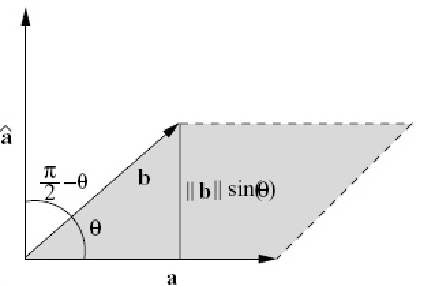
\includegraphics[height=2in]{2_ppgram2}}
\caption{The vector $a^\perp$ (labelled incorrectly in the figure as $\hat{a}$). \label{fig_ppgram2}}
\end{figure}

Using the geometric meaning of the dot product, we obtain
\begin{eqnarray*}
\det\left[\matrix{a_1&a_2\cr b_1&b_2\cr}\right]
 & = & \aa^\perp\cdot\bb \\
 & = & \|\aa^\perp\|\|\bb\|\cos(\pi/2-\theta) \\
 & = & \|\aa\|\|\bb\|\sin(\theta)
\end{eqnarray*}
We need to be a bit careful here.  When we were discussing the dot
product, we always assumed that the angle between two vectors was in
the range $0$ to $\pi$.  In fact, the geometric formula for the dot
product is not sensitive to how we measure the angle. Suppose that
instead of $\theta$ in the range $0$ to $\pi$ we use
$\theta_1=-\theta$ (measuring the angle ``backwards'') or
$\theta_2=2\pi-\theta$ (measuring the angle going the long way around
the circle). Since $\cos(\theta)=\cos(-\theta)=\cos(2\pi-\theta)$ we
have
\[ \cc\cdot\dd=\|\cc\|\|\dd\|\cos(\theta)=\|\cc\|\|\dd\|\cos(\theta_1)
=\|\cc\|\|\dd\|\cos(\theta_2).
\]
In other words, the geometric formula for the dot product still is
true.

In the diagram above, we want to let the angle $\theta$ between $\aa$
and $\bb$ range between $-\pi$ and $\pi$.  In this case the angle
$\pi/2-\theta$ between $\aa^\perp$ and $\bb$ is sometimes not in the
range between $0$ or $2\pi$. But if this happens, then it is still the
angle between $\aa^\perp$ and $\bb$, just ``backwards'' or ``the long
way around.'' Thus the geometric formula above still is correct.

Values of $\theta$ between $0$ and $\pi$ correspond to the situation
where the direction of $\bb$ is obtained from the direction of $\aa$
by a counterclockwise rotation of less than $\pi$. This is the case in
the diagram. On the other hand, $\theta$ between $-\pi$ and $0$
corresponds to the case where a clockwise rotation of less than $\pi$
is needed to get from the direction of $\aa$ to the direction of
$\bb$.

The quantity $\sin(\theta)$ can be positive or negative, depending on
the orientations of $\aa$ and $\bb$, but in any case the positive
quantity $\|\bb\||\sin(\theta)|$ is the height of the parallelogram
spanned by $\aa$ and $\bb$ if we take $\aa$ to be the base. In this
case, the length of the base is $\|\aa\|$. Recall that the area of a
parallelogram is the length of the base times the height. Thus
\[
\left|\det\left[\matrix{a_1&a_2\cr b_1&b_2\cr}\right]\right|
=\hbox{Area of parallelogram spanned by $\aa$ and $\bb$}
\]
The determinant is positive if $\sin(\theta)$ is positive, that is, if
$\theta$ is positive. This is the case if the direction of $\bb$ is
obtained by a counterclockwise rotation of half a circle or less from
the direction of $\aa$. Otherwise the determinant is negative.

Notice that the determinant whose rows are the components of two
non-zero vectors $\aa$ and $\bb$ is zero exactly when the vectors
$\aa$ and $\bb$ are pointing in the same direction, or in the opposite
direction, that is, if one is obtained from the other by scalar
multiplication.  The sign of the determinant gives information about
their relative orientation.

\begin{example}
Find the area $\cal A$ of the parallelogram spanned by $\aa = [1, 1]$ and 
$\bb = [1, 3]$. {\rm 
Using the formula above, we know that 
\[
{\cal A} = \left|\det\left[\matrix{1 & 1 \cr 1 & 3\cr}\right]\right| 
= | 3-1| = |2| = 2.
\]
In addition, since the determinant is positive, we know that $\bb$ is counterclockwise to $\aa$ 
as can be seen graphically. 
}
\end{example} 

\subsection{The cross product}

Unlike the dot product, the cross product is only defined for vectors
in three dimensions. And unlike the dot product, the cross product of
two vectors is another vector, not a number. If $\aa = [a_1,a_2,a_3]$
and $\bb=[b_1,b_2,b_3]$, then $\aa \times \bb$ is a vector given by
\[
\aa \times \bb = [a_2b_3-a_3b_2, a_3b_1-a_1b_3, a_1b_2-a_2b_1].
\]
An easy way to remember this is to write down a $3\times 3$ matrix whose
first row contains the unit basis vectors and whose second and third rows
contain the components of $\aa$ and $\bb$. Then the cross product is obtained
by following the usual rules for computing a $3\times 3$ determinant.
\begin{eqnarray*}
\det\left[\matrix{
	{\bf i}&{\bf j}&{\bf k}\cr
	a_1&a_2&a_3\cr
	b_1&b_2&b_3\cr
}\right]
  & = & {\bf i}\det\left[\matrix{a_2&a_3\cr b_2&b_3\cr}\right]
- {\bf j}\det\left[\matrix{a_1&a_3\cr b_1&b_3\cr}\right]
+ {\bf k}\det\left[\matrix{a_1&a_2\cr b_1&b_2\cr}\right] \\
  & = & [a_2b_3-a_3b_2, a_3b_1-a_1b_3, a_1b_2-a_2b_1]
\end{eqnarray*}
The geometric meaning of the cross product is given
the following three properties:
\begin{enumerate}
\item $\aa\times\bb$ is orthogonal to $\aa$ and to $\bb$
\item $\|\aa\times\bb\|=\|\aa\|\|\bb\|\sin(\theta)$, where $\theta$ is
the angle between $\aa$ and $\bb$. In this formula, $\theta$ lies
between $0$ and $\pi$, so that $\sin(\theta)$ is positive.  This is
the same as saying that the length of $\aa\times\bb$ is the area of
the parallelogram spanned by $\aa$ and $\bb$.
\item The vectors $\aa$, $\bb$ and $\aa\times\bb$ obey the right hand
rule.
\end{enumerate}
This geometric description of the cross product shows that the
definition of the cross product is independent of how we choose our
co-ordinate axes.  To verify 1, we compute the dot products
$\aa\cdot(\aa\times\bb)$ and $\bb\cdot(\aa\times\bb)$ and verify that
they are zero. (This is one of the problems below.)

To verify 2 we must show that the length of $\aa\times\bb$ is the area
of the parallelogram spanned by $\aa$ and $\bb$, since the quantity
$\|\aa\|\|\bb\|\sin(\theta)$ is precisely this area.

Since both the length and the area are positive quantities, it is
enough to compare their squares. We have 
\begin{equation}
\label{cross1}
\|\aa\times\bb\|^2 =
(a_2b_3-a_3b_2)^2+(a_3b_1-a_1b_3)^2+(a_1b_2-a_2b_1)^2
\end{equation}

On the other hand, the area $A$ of the parallelogram spanned by $\aa$ and
$\bb$ is length $\|\aa\|$ times the height. This height is the length
of the vector $\bb-{\rm proj}_{\aa}\bb = \bb - (\aa\cdot\bb)\aa/\|\aa\|^2$
as shown in Figure~\ref{fig_ppgram}.
Using these facts, we arrive at the following formula for the square
of the area of the parallelogram. 

\begin{figure}
\centerline{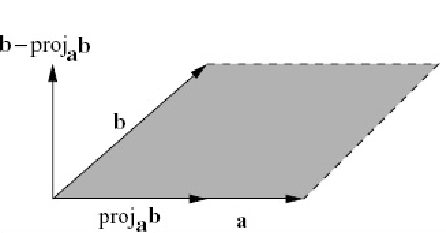
\includegraphics[height=2in]{2_ppgram}}
\caption{The parallelogram spanned by $\aa$ and $\bb$. \label{fig_ppgram}}
\end{figure}

\begin{eqnarray}
\nonumber 
A^2 & = & \|\aa\|^2\| \bb - (\aa\cdot\bb)\aa/\|\aa\|^2\|^2 \\
\nonumber 
    & = & \|\aa\|^2\left(
          \|\bb\|^2 + (\aa\cdot\bb)^2\|\aa\|^2/\|\aa\|^4 -
          2(\aa\cdot\bb)^2/\|\aa\|^2\right) \\
\nonumber 
    & = & \|\aa\|^2\|\bb\|^2 - (\aa\cdot\bb)^2 \\
\label{cross2}
    & = & (a_1^2+a_2^2+a_3^2)(b_1^2+b_2^2+b_3^2)-(a_1b_1+a_2b_2+a_3b_3)^2
\end{eqnarray}
Expanding the expressions in (\ref{cross1}) and (\ref{cross2}) reveals
that they are equal.

Notice that there are exactly two vectors satisfying properties 1 and
2, that is, perpendicular to the plane spanned by $\aa$ and $\bb$ and
of a given length. The cross product of $\aa$ and $\bb$ is the one
that satisfies the right hand rule. We say that vectors $\aa$, $\bb$
and $\cc$ (the order is important) satisfy the right hand rule if you
can point the index finger of your right hand in the direction of
$\aa$ and the middle finger in the direction of $\bb$ and the thumb in
the direction of $\cc$.  Try to convince yourself that if $\aa$, $\bb$
and $\cc$ (in that order) satisfy the right hand rule, then so do
$\bb$, $\cc$, $\aa$ and $\cc$, $\aa$, $\bb$.

Here are some properties of the cross product that are useful in doing
computations. The first two are maybe not what you expect.
\begin{enumerate}
\item $\aa\times\bb=-\bb\times\aa$
\item $\aa\times(\bb\times\cc)=(\cc\cdot\aa)\bb-(\bb\cdot\aa)\cc$.
\item $s(\aa\times\bb)=(s\aa)\times\bb=\aa\times(s\bb)$.
\item $\aa\times(\bb+\cc) = \aa\times\bb + \aa\times\cc$.
\item $\aa\cdot(\bb\times\cc)=(\aa\times\bb)\cdot\cc$.
\end{enumerate}

\begin{example}
\label{2008_a2_2} Let $\aa = (1,3,-2)$ and $\bb = (-1,2,3)$. Compute
the following:
{\begin{enumerate}
\renewcommand{\labelenumi}{(\alph{enumi})}
\item The area of the parallelogram whose sides are $\aa$ and $\bb$. 
\item The angle between $\aa$ and $\bb$. 
\end{enumerate}}
{\rm Solution:
\begin{enumerate}
\renewcommand{\labelenumi}{(\alph{enumi})}
\item The area of the parallelogram is equal to the length of 
$\aa \times \bb$:
\[
\aa \times \bb =  \left| \begin{array}{ccc}
\hat{i} & \hat{j} & \hat{k} \\
1 & 3 & -2 \\
-1 & 2 & 3
\end{array} \right| = \hat{i} (9+4) + \hat{j} (2-3) + \hat{k}(2+3) 
   = (13,-1,5) 
\]
so the area is 
\[
\| \aa \times \bb \| = \sqrt{13^2 + (-1)^2 + 5^2} = \sqrt{195} 
   \approx 13.96
\]
\item Note that the formula 
$\| \aa \times \bb \| = \| \aa \| \| \bb \| \sin \theta$ cannot be used 
for this question since it cannot distinguish between $\theta$ and 
$\pi - \theta$ (think about this point). Instead, use the $\cos$, dot 
product formula which should always be used for the calculation of 
angles between vectors unless you really know what you are doing:
\[
\cos \theta = \frac{\aa \cdot \bb}{\| \aa \| \| \bb \|} = 
\frac{(1,3,-2)\cdot (-1,2,3)}{\|(1,3,-2)\| \|(-1,2,3)\|} 
= \frac{-1+6-6}{\sqrt{1+9+4} \sqrt{1+4+9}} = \frac{-1}{14} 
\]
so 
\[
\theta = \cos^{-1} \left( \frac{-1}{14} \right) \approx 1.64 
   \mbox{\ radians or $\approx 94.10^\circ$}
\]
\end{enumerate}}
\end{example}

\begin{example}
Consider the triangle $T$ with three corners $(1,1,1)$, $(1,2,3)$ and $(2,0,1)$. Find the 
area of $T$. 
{\rm The area will be half of the area of the parallelogram spanned by (any) two 
distinct sides. We take sides $(1,2,3)-(1,1,1) = (0,1,2)$ and $(2,0,1) -(1,1,1) = (1,-1,0)$
which make the computations a bit easier. We compute 
\[
(0,1,2) \times (1,-1,0) = \det \left[ \begin{array}{ccc}
\hat{i} & \hat{j} & \hat{k} \\
0 & 1 & 2 \\
1 & -1 & 0
\end{array} \right] = (2, 2,-1) 
\]
and then the area of the triangle is 
\[
1/2 \| (2,2,-1) \| = 3/2. 
\] 
} 
\end{example} 
Try to convince yourself why it does not matter which two sides are taken in the computation above. 

\subsection{The triple product and the determinant in three dimensions}

The cross product is defined so that the dot product of $\aa$ with
$\bb\times\cc$ is a determinant:
\[
\aa\cdot(\bb\times\cc) = 
\det\left[\matrix{
	a_1&a_2&a_3\cr
	b_1&b_2&b_3\cr
	c_1&c_2&c_3\cr
}\right]
\]
This determinant is called the triple product of $\aa$, $\bb$ and
$\cc$.

Using this fact we can show that the absolute value of the triple
product is the volume of the parallelepiped spanned by $\aa$, $\bb$
and $\cc$.

A diagram of the parallepiped is shown in Figure~\ref{fig_triple}. 
The absolute value of the triple product is
\[
\left|\aa\cdot(\bb\times\cc)\right|
  = \|\aa\|\cos(\theta)\|\bb\times\cc\|.
\]
Here $\theta$ is the angle between $\aa$ and $\bb\times\cc$.
The quantity $\|\aa\|\cos(\theta)$ is the height of parallelepiped and
$\|\bb\times\cc\|$ is the area of the base. The product of these is
the volume of the parallepiped, as claimed. Thus
\[
\left|\det\left[\matrix{
	a_1&a_2&a_3\cr
	b_1&b_2&b_3\cr
	c_1&c_2&c_3\cr
}\right]\right|
=\mbox{Volume of the parallelepiped spanned by $\aa$, $\bb$ and $\cc$}
\]

\begin{figure}
\centerline{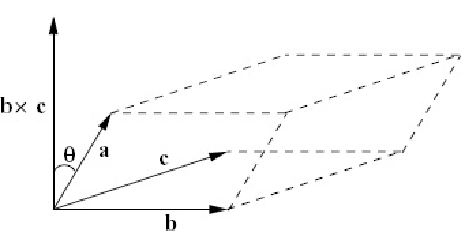
\includegraphics[height=2in]{2_triple}}
\caption{The Triple Product. \label{fig_triple}}
\end{figure}

The sign of the triple product is positive if $\theta$ is between
zero and $\pi/2$ and negative if $\theta$ lies between $\pi/2$ and
$\pi$.  This is the case if $\aa$ is on the same side of the plane
spanned by $\bb$ and $\cc$ as $\bb\times\cc$. This holds if the
vectors $\bb$, $\cc$ and $\aa$ (in that order) satisfy the right hand
rule. Equivalently $\aa$, $\bb$ and $\cc$ (in that order) satisfy the
right hand rule.

Mathematically, it is more satisfactory to define the right hand rule
using the determinant. That is, we say that vectors $\aa$, $\bb$ and
$\cc$ satisfy the right hand rule if the determinant
$\aa\cdot(\bb\times\cc)$ is positive.

\subsection{MATLAB: assigning matrices and {\tt det} and {\tt cross} 
commands}

\begin{description}
\item[{\tt cross}] The command {\tt cross(a,b)} computes the cross 
product $\aa \times \bb$. An error results if {\tt a} or {\tt b} are not 
vectors of length 3. As an example, the command
\begin{verbatim}
cross([1 0 0],[0 1 0])
\end{verbatim} 
gives the vector result [0 0 1]. 
\item[{\bf matrices:}] The syntax to generate a matrix is shown below using 
a $2 \times 2$ example
\begin{verbatim}
a = [1 2; 3 4]
\end{verbatim}
This command assigns a matrix to {\tt a} that has the vector [1 2] in its 
first row and [3 4] in its second. Entries of a matrix can be accessed 
individually, for example {\tt a(1,2)} is the entry in the first row, 
second column. 
\item[{\tt zeros}:] Many applications can lead to large 
matrices with many rows and columns. Even though MATLAB can do matrix 
computations, it can be tedious to enter these large matrices by hand. 
In some cases the matrices have mostly zeros as entries (these matrices 
are called {\em sparse}). In these cases it is more efficient to generate 
a matrix of all zeros and then modify the entries that are not zero. 
For example 
\begin{verbatim}
a = zeros(2,2);
a(1,1) = 1;
\end{verbatim}
generates a $2 \times 2$ matrix with entries that are all zero except the 
upper left entry which is 1. Note that {\tt zeros(n,m)} generates a 
matrix with $n$ rows and $m$ columns with all zero entries. 
So {\tt zeros(1,m)} is a row vector of length $m$ and {\tt zeros(n,1)}
is a column vector of length $m$ with all zero entries. 
\item[{\tt rand}:] {\tt rand (n,m)} generates a 
matrix with $n$ rows and $m$ columns with entries that are random numbers 
uniformly distributed in the interval [0,1].  
\item[{\tt det}:] The command {\tt det(a)} returns the determinant 
of the matrix {\tt a}. An error occurs if {\tt a} is not 
a square (same number of rows and columns) matrix. Determinants of 
larger matrices (than $2 \times 2$ and $3 \times 3$ discussed in this
section) are discussed in Chapter~\ref{ch_matrices_dets}.
\end{description}

\subsection{MATLAB: generating scripts with the MATLAB editor}

Often times using the command window in MATLAB to solve a problem can be tedious, because if the need arises to redo the problem, or change a parameter, one has to rewrite it all. The editor comes in handy for such cases. The editor is a text window (accessed from the command window: {\tt File $\rightarrow$ New $\rightarrow$ Blank M-file}) where one can write commands in the same syntax as the editor, and when one runs it, the results appear in the command window exactly as if one had written them there one after the other.

For example, the code to generate three random orthogonal vectors would look something like this:
\begin{verbatim}
a1 = rand(3,1)
b = rand(3,1);
a2 = cross(a1,b)
a3 = cross(a1,a2)
dot(a1,a2)
dot(a1,a3)
dot(a2,a3)
\end{verbatim}
Note that the last three lines are there to check that the three vectors are mutually orthogonal. Once the code was written, save it from the editor window: {\tt File $\rightarrow$ Save as}, making sure that the name of the file has a ``{\tt .m}'' extension (and the file name should contain no spaces). There are several different ways of running the script, the fastest one is to hit the {\tt F5} key. Alternatively, from the editor window it can be run from {\tt Debug $\rightarrow$ Run}, or directly from the command window by typing the name of the script into the MATLAB command line.

\subsection{MATLAB: floating point representation of real numbers}
\label{sec:floating}

MATLAB can represent integers exactly (up to limited but large size). Using a 
``floating point representation", MATLAB can represent 
most real numbers only approximately (but quite accurately - to 16 digits or so). In certain 
cases, the errors made in floating point approximation of numbers can be amplified 
and lead to noticeable errors in computed results. This will not happen typically in the 
examples and computer labs for Math 152, but the reader should be aware of the possibility. 

\begin{example} Consider the vectors 
\begin{eqnarray*}
{\bf a} & = & [1 \; 1 \; 1] \\
{\bf b} & = & [\sqrt{2} \; \sqrt{2} \; 0]
\end{eqnarray*}
and ${\bf c} = {\bf a} + {\bf b}$. 
If a $3 \times 3$ matrix $A$  is made with rows ${\bf a}$, ${\bf b}$ and ${\bf c}$ then 
the determinant of $A$ is zero (by construction, the vectors lie on the same plane). 
If this computation is done in MATLAB, 
\begin{verbatim}
a = [1 1 1];
b = [sqrt(2) sqrt(2) 0 ];
c = a + b;
A = [a; b; c];
det(A)
\end{verbatim}
the result is 3.1402e-16 not zero due to floating point approximation of intermediate 
computations. You can type {\tt eps} in MATLAB to see the maximum 
relative error made by 
floating point approximation. On the computer used to do the computation above, 
{\tt eps} had a value of 2.2204e-16, so it is believable that the calculation error in 
the determinant was made by the combination of a few floating point   approximations.
\end{example} 

Try to determine how many decimal digits of accuracy the floating point representation 
in your calculator uses (typically, the accuracy is greater than what is displayed). 

\subsection{Problems}

\begin{problem}
\label{op1_12}
Compute $[1,2,3]\times[4,5,6]$
\end{problem}

\begin{problem}
\label{2009_a2_1}
Use the definition to find the determinant of the matrix
\[
\left[ \begin{array}{ccc}
1 & 1 & 1 \\
1 & 2 & 3 \\
1 & 0 & -1
       \end{array} \right].
\]
Do the computation by hand showing your work, but you can check
your result using MATLAB.
From your result, decide if the vectors [1 1 1], [1 2 3] and [1 0 -1]
lie in the same plane (justify your answer, very briefly).
\end{problem}

\begin{problem}
\label{op1_13}
Verify that $\aa\cdot(\aa\times\bb)=0$ and $\bb\cdot(\aa\times\bb)=0$.
\end{problem}

\begin{problem}
\label{2008_a2_1} Simplify each of the following expressions:
{\begin{enumerate}
\renewcommand{\labelenumi}{(\alph{enumi})}
\item $((1,4,-1)\cdot(2,1,3)) ((2,1,4) \times (1,4,9))$
\item $(7,1,0)\cdot ((2,0,-1) \times (1,4,3))$
\item $(\aa \times \bb) \times (\bb \times \aa)$
\end{enumerate}}
\end{problem}

\begin{problem}
\label{op1_14}
Explain why $\|\aa\|\|\bb\|\sin(\theta)$ is the area of the
parallelogram spanned by $\aa$ and $\bb$. Here $\theta$ is the angle
between the two vectors.
\end{problem}

\begin{problem}
\label{op1_15}
Find examples to show that in general $\aa\times\bb\ne\bb\times\aa$
and $\aa\times(\bb\times\cc)\ne(\aa\times\bb)\times\cc$.
\end{problem}

\begin{problem}
\label{matlab_op1_15}
(Matlab) The Matlab command {\tt a=rand(1,n)} generates an $n\times 1$ vector with random entries. Write a script that generates three random vectors and write what you obtain from $\aa\times\bb-\bb\times\aa$,
and from $\aa\times(\bb\times\cc)-(\aa\times\bb)\times\cc$. Does that constitute a proof?
\end{problem}

\begin{problem}
\label{op1_16}
Show that $\aa\times(\bb\times\cc)=(\aa\cdot\cc)\bb-(\aa\cdot\bb)\cc$.
\end{problem}

\begin{problem}
\label{matlab_op1_16}
(Matlab) Write a script that generates three random vectors and checks that the result from problem \ref{op1_16} holds: $\aa\times(\bb\times\cc)=(\aa\cdot\cc)\bb-(\aa\cdot\bb)\cc$.
\end{problem}

\begin{problem}
\label{op1_17}
Derive an expression for $(\aa\times\bb)\cdot(\cc\times{\bf d})$ that
involves dot products but not cross products.
\end{problem}

\begin{problem}
\label{2008_a2_5}
{\begin{enumerate}
\renewcommand{\labelenumi}{(\alph{enumi})}
\item Draw a sketch containing the vectors $\aa$, $\bb$ and 
$\aa \times (\aa \times \bb)$. Assume that $\aa$ and $\bb$ lie in the 
plane of the paper and have an acute angle between them. 
\item Find a formula for $\aa \times (\aa \times \bb)$ which 
involves only $\| a \|$, $\bb$ and $\mbox{proj}_\aa \bb$. {\em Hint:} 
use a property of the dot product. 
\end{enumerate}}
\end{problem}

\begin{problem}
\label{op1_18}
What is the analog of the cross product in two dimensions? How about
four dimensions?
\end{problem}

\section{Lines and Planes} 

\subsection{Describing linear sets}

The following sections we will consider points, lines, planes and space
in two and three dimensions. Each of these sets have two complementary (or dual)
descriptions. One is is called the parametric form and the other the equation
form. Roughly speaking, the parametric form specifies the set using vectors
that are parallel to the set, while the equation form uses vectors that are
orthogonal to the set. Using the parametric description, it is easy to 
write down explicitly all the elements of the set, but difficult to check
whether a given point lies in the set. Using the equation description its the
other way around: if someone gives you a point, it is easy to check whether it
lies in the set, but it is difficult to write down explicitly even a single
member of the set. 

One way of thinking about solving a system of linear equations is simply going
from one description to the other. This will (hopefully) become clear later on.

These sections will always follow the same pattern. We will consider the
parametric and equation descriptions, first in the
special case when the set passes through the origin. Then we consider the
general case. 
Recall that when we say ``the point $\xx$'' this means ``the point at the head
of the vector $\xx$ whose tail is at the origin.''
In these sections we have used the notation $[x_1,x_2]$ instead of $[x,y]$ 
and $[x_1,x_2,x_3]$ instead of $[x,y,z]$ for typical points in two and three
dimensions.

\subsection{Lines in two dimensions: Parametric form}

First we consider lines passing through the origin.
Let $\aa=[a_1,a_2]$ be 
vector in the direction of the line. Then all the points $\xx$ on the line
are of the form 
\[
\xx = s\aa
\]
for some number $s$. The number $s$ is called a 
parameter. Every value of $s$ corresponds to exactly one point (namely $s\aa$) 
on the line.

Now we consider the general case. Let $\qq$ be a point on the line and $\aa$
lie in the direction of the line. Then the points on the line can be thought of
as the points on the line through the origin in the direction of $\aa$ shifted
or translated by $\qq$. Then a point $\xx$ lies on the line through
$\qq$ in the direction of $\aa$ exactly when 
\[
\xx=\qq+s\aa
\]
for some value of $s$.

\begin{example}
Find a parametric form of the line that goes through the points (1,2) and (2,4). 
{\rm We find the direction vector from 
\[
(2,4) - (1,2) = (1,2). 
\] 
Now 
\[
(1,2) + s (1,2) 
\]
is a parametric form of the line. That is, every point on the line can be written in the form above with a (unique) value of $s$ and every point of the form above is on the line. Note that parametric forms are not unique. The same line can be described by 
\[
(2,4) + t (2,4) 
\]
since we know the point (2,4) is on the line and the direction (2,4) is a scalar multiple of (1,2). Of course, specific points on the line will correspond to different values of $s$ and $t$. 
}
\end{example}



\subsection{Lines in two dimensions: Equation form}

First we consider lines passing through the origin shown in 
Figure~\ref{fig_line2d} (left).
Let $\bb=[b_1,b_2]$ be orthogonal to the direction of line. 
The point $\xx$ is on 
the line exactly when $\xx\cdot\bb=0$. This can be written
\[
x_1b_1 + x_2b_2 = 0.
\]

Now we consider the general case shown in 
Figure~\ref{fig_line2d} (right).
Let $\qq$ be a point on the line and
$\bb=[b_1,b_2]$ be orthogonal to the direction of line. A point $\xx$ lies on
the line through $\qq$ in the direction of $\aa$ exactly when $\xx-\qq$ lies
on the line through the origin in the direction of $\aa$. Thus
$(\xx-\qq)\cdot\bb =0$. This can be written
\[
(x_1-q_1)b_1 + (x_2-q_2)b_2 = 0
\]
or
\[
x_1b_1 + x_2b_2 = c,
\]
where $c=\qq\cdot\bb$. 

\begin{figure}
\centerline{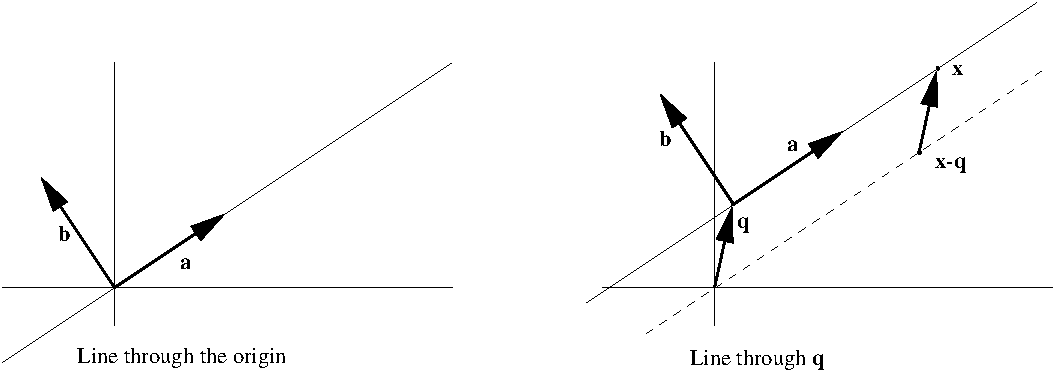
\includegraphics[height=1.5in]{2_line2d}}
\caption{A line in two dimensions. \label{fig_line2d}}
\end{figure}

\begin{example}
Find an equation form for the line in parametric form below:
\[
(1,2) + s (1,2).
\] 
{\rm We need to find a vector perpendicular to (1,2). We use the idea from section~\ref{s:trick}
and use 
\[
(1,2)^\perp = (-2,1) 
\]
Together with the point (1,2) on the line, we have an equation form 
\[
-x_1 + 2x_2 = (-2,1) \cdot (1,2) = 0 
\]
}
\end{example}

\begin{example} 
Find a parametric form for the line in equation form below:
\begin{equation}
\label{eq:2deqline} 
x_1 + 4 x_2 = 1. 
\end{equation} 
{\rm We need to find a point (any point) on the line. It is simple to look for the $x_2$ intercept ($x_2=0$) and find the point (1,0). The direction of the line will be perpendicular to (1,4) so we will use 
\[
(1,4)^\perp = (-4,1) 
\]
to get the parametric form 
\[
(x_1, x_2) = (1,0) + s(-4,1) 
\]
Note that for every $s$ we get a point that satisfies (\ref{eq:2deqline}). 
}
\end{example} 

\subsection{Lines in three dimensions: Parametric form}

The parametric form of a line in three (or higher) dimensions looks just
the same as in two dimensions. The points $\xx$ on the line are 
obtained by starting at
some point $\qq$ on the line and then adding all multiples 
of a vector $\aa$ pointing in the direction of the line. So
\[
\xx=\qq+s\aa
\]
The only difference is
that now $\qq$ and $\aa$ are vectors in three dimensions.

\begin{example} Find a parametric form for the line that passes through (1,1,1) and 
(1,2,3). Determine if the point (1,-2,3) is on the line. 
{\rm We find the direction of the line 
\[
(1,2,3) -(1,1,1) = (0,1,2) 
\]
so a parametric form of the line is 
\[
(1,1,1) + s(0,1,2). 
\]
If (1,-2,3) were on the line then 
\[
(1,1,1) + s(0,1,2) = (1,-2,3) 
\]
for some $s$. The above is a vector equation that must be satisfied for every component. The first component reads $1+0\times s = 1$ which is true for all $s$. The second component 
reads $1+s = -2$ which requires $s=-3$. If we now check the third component $1-3(2) = -5 \neq 3$. We conclude that (1,-2,3) is not on the line. 
}
\end{example}

\subsection{Lines in three dimensions: Equation form}

We begin with lines through the origin. A line through the origin can be
described as all vectors orthogonal to a plane. Choose two
vectors $\bb_1$ and $\bb_2$ lying in the plane that are not collinear (or zero).
Then a vector is orthogonal to the plane if and only if it is orthogonal to both
$\bb_1$ and $\bb_2$. Therefore the line consists of all points $\xx$ such that
$\xx\cdot\bb_1=0$ and $\xx\cdot\bb_2=0$. 
If $\bb_1=[b_{1,1},b_{1,2},b_{1,3}]$ and
$\bb_2=[b_{2,1},b_{2,2},b_{2,3}]$ then these equations can be written
\[
\matrix{
b_{1,1}x_1 &+ &b_{1,2}x_2 &+ &b_{1,3}x_3&= &0\cr
b_{2,1}x_1 &+ &b_{2,2}x_2 &+ &b_{2,3}x_3&= &0\cr
}
\]
Notice that there are many possible choices for the vectors $\bb_1$ and $\bb_2$.
The method of Gaussian elimination, studied later in this course, is a method of
replacing the vectors $\bb_1$ and $\bb_2$ with equivalent vectors in such a way
that the equations become easier to solve. 

Now consider a line passing through the point $\qq$  
and orthogonal to the directions
$\bb_1 $ and $\bb_2$ as shown in Figure~\ref{fig_line3d}. 
A point $\xx$ lies on this line precisely when $\xx-\qq$
lies on the line through the origin that is orthogonal to $\bb_1 $ and $\bb_2$.
Thus $(\xx-\qq)\cdot\bb_1=0$ and $(\xx-\qq)\cdot\bb_2=0$. This can be written
\[
\matrix{
b_{1,1}(x_1-q_1) &+ &b_{1,2}(x_2-q_2) &+ &b_{1,3}(x_3-q_3)&= &0\cr
b_{2,1}(x_1-q_1) &+ &b_{2,2}(x_2-q_2) &+ &b_{2,3}(x_3-q_3)&= &0,\cr
}
\]
or
\[
\matrix{
b_{1,1}x_1 &+ &b_{1,2}x_2 &+ &b_{1,3}x_3&= &c_1\cr
b_{2,1}x_1 &+ &b_{2,2}x_2 &+ &b_{2,3}x_3&= &c_2\cr
}
\]
where $c_1=\qq\cdot\bb_1$ and $c_2=\qq\cdot\bb_2$

\begin{figure}
\centerline{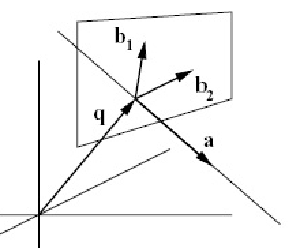
\includegraphics[height=2in]{2_line3d}}
\caption{A line in three dimensions. \label{fig_line3d}}
\end{figure}

\begin{example}
\label{ex:convert} 
Find a parametric and an equation form of the line that passes through the points (0,1,5) and (2,2,2).
{\rm We find a direction vector 
\[
{\bf v} = (2,2,2)-(0,1,5) = (2,1,-3)
\]
and write a parametric form for the line 
\[
{\rm \bf L:} {\bf x} = (0,1,5) + s(2,1,-3).
\]
To write an equation form we need to find two {\em different} (not collinear) vectors perpendicular to $\bf v$. To get one, we can use a variant of the procedure in Section~\ref{s:trick} where we rotated 2D vectors by 90$^\circ$ to get a perpendicular vector. 
\[
{\bf b_1} = (0, 3, 1).
\]
You can check directly that $\bf b_1$ is perpendicular to $\bf v$ (${\bf b_1} \cdot {\bf v} = 0$). To get the second vector $\bf b_2$ we can use the same idea on different components:
\[
{\bf b_2} = (-1,2,0).
\]
Note that ${\bf b_2}$ is perpendicular to $\bf v$ and not a multiple of $\bf b_1$ as required.  
An alternative for the second vector would be ${\bf b_1} \times \bf v$ since that vector is perpendicular to both $\bf v$ and $\bf b_1$. With the formulas above, we can write an equation form for the line:
\[
\matrix{
 & &3 x_2 &+ &x_3&= &8 \cr
-x_1 &+ &2x_2 & & &= &2.\cr
}
\]
You can check your answer by showing that both of the original points satisfy both equations. }
\end{example} 

\subsection{Planes in three dimensions: Parametric form}

We begin with planes through the origin. Since a plane is a two dimensional
object, we will need two parameters to describe points on the plane. Let $\aa_1$
and $\aa_2$ be non-collinear vectors in the direction of the plane. Then every
point on the plane can be reached by adding some multiple of $\aa_1$ to some
other multiple of $\aa_2$. In other words, points $\xx$ on the plane are 
all points of the form 
\[
\xx=s\aa_1+t\aa_2
\]
for some values of $s$ and $t$. 

If the plane passes through some point $\qq$ in the directions of $\aa_1$
and $\aa_2$, then we simply shift all the points on the parallel plane through
the origin by $\qq$. So $\xx$ lies on the plane if
\[
\xx=\qq+s\aa_1+t\aa_2
\]
for some values of $s$ and $t$. 

\begin{example} Find a parametric form of the plane that passes through the points (1,0,0), (1,1,1) and 
(1,0,2).
{\rm We find direction vectors 
\begin{eqnarray*}
{\bf a_1}  & = & (1,1,1)-(1,0,0) = (0,1,1) \\
{\bf a_2} & = & (1,0,2) - (1,0,0) = (0,0,2). 
\end{eqnarray*}
Note that $\bf a_1$ and $\bf a_2$ do not have the same direction (are not collinear). If they had been, then the three points would all be on the same line and so would not define a unique plane. We can proceed with the parametric form of the plane
\[
{\bf x} = (1,0,0) + s {\bf a_1} + t {\bf a_2} = (1, s, s+2t).
\]
}
\end{example}

\subsection{Planes in three dimensions: Equation form}

A plane through the origin can be described as all vectors orthogonal 
to a given vector $\bb$ as shown in Figure~\ref{fig_plane3d}. 
(In this situation, if $\bb$ has unit length it is called 
the normal vector to the plane and is often denoted ${\bf n}$.)
Therefore $\xx$ lies on the plane whenever $\xx\cdot\bb=0$, or
\[
\matrix{
b_{1}x_1 &+ &b_{2}x_2 &+ &b_{3}x_3&= &0.\cr
}
\]
If a plane with normal vector $\bb$ is translated so that it passes 
through the point $\qq$, then $\xx$
lies on the plane whenever $\xx-\qq$ lies on the parallel plane through the
origin. Thus $\xx$ lies on the plane whenever $(\xx-\qq)\cdot\bb=0$.
Equivalently
\[
\matrix{
b_{1}(x_1-q_1) &+ &b_{2}(x_2-q_2) &+ &b_{3}(x_3-q_3)&= &0,
}
\]
or
\[
\matrix{
b_{1}x_1 &+ &b_{2}x_2 &+ &b_{3}x_3&= &c,
}
\]
where $c=\qq\cdot\bb$.

\begin{figure}
\centerline{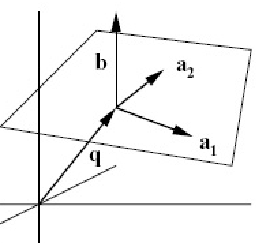
\includegraphics[height=2in]{2_plane3d}}
\caption{A plane in three dimensions. \label{fig_plane3d}}
\end{figure}

\begin{example}
Write the equation form of the plane described by the parametric form below:
\[
{\bf x} = (1+s+t, 5t, -2) 
\]
{\rm {\em Note:} It is possible to see the answer from the form above, but let us go through the steps of the calculations you would do if the example were more complicated. Write the expression above as 
\[
{\bf x} = (1,0,-2) + s(1,0,0) + t (1,5,0).
\]
In this form we can recognize ${\bf q} = (1,0,-2)$ as a point on the plane (corresponding to parameters $s=0$ and $t=0$) and the vectors ${\bf a}_1 = (1,0,0)$ and ${\bf a}_2 = (1,5,0)$ as directions {\em in} the plane. To write the equation form of the plane, we need a point on it (which we have) and the normal direction $\bf b$ to it, which must be perpendicular to ${\bf a}_1$ and ${\bf a}_2$. Thus we can compute 
\[
{\bf b} = {\bf a}_1 \times {\bf a}_2 = (0, 0, 5).
\]
Now the equation form of the plane is ${\bf b} \cdot {\bf x} = {\bf b} \cdot {\bf q}$ :
\[
0x + 0y + 5z = 0\cdot 1 + 0 \cdot 1 + 5 \cdot -2 = -10 
\mbox{\ \ \ or $z=-2$}   
\]
where in this case we have written the components of the vector $\bf x$ as $(x,y,z)$. }
\end{example} 

\begin{example}
Find a parametric form for the plane $x + y + 2z = 2$.
{\rm We identify the normal direction to the plane ${\bf b} = (1,1,2)$ by inspection. We need a point on the plane. It is easy to find one on the coordinate axes, (2,0,0) for example. To get two directions $\bf a_1$ and $\bf a_2$ in the plane, we need two different directions perpendicular to $\bf b$. Proceeding as in Example~\ref{ex:convert} we take 
\[
{\bf a_1} = (0,-2,1) \mbox{\ and \ } {\bf a_2} = (-1,1,0)
\]
leading to a parametric form 
\[
{\bf x} = (1,0,0) +s {\bf a_1} + t {\bf a_2} = (1-t, -2s+t, s) .
\]
}
\end{example}

\subsection{Problems}

\begin{problem}
\label{op1_21}
A line orthogonal to $\bb$ can be described as the set of all points $\xx$
whose projections onto $\bb$ all have the same value.
Using the formula for projections, show that this leads to the
equation description of the line.
\end{problem}

\begin{problem}
\label{op1_22}
Find both the parametric form and equation form for the line in Figure 
\ref{fig_lineprob}.
Write down five points on the line (notice that the parametric form is 
more useful for this). Check whether the point 
$[{{1012}\over{3}},{{1069}\over{21}}]$ is on the line
(notice that the equation form is more useful for this.)
\end{problem}

\begin{figure}
\centerline{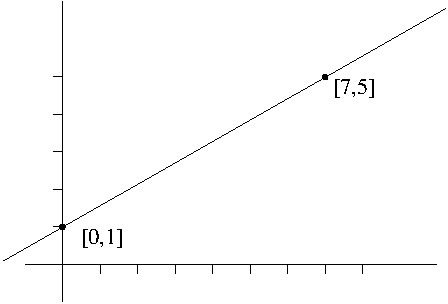
\includegraphics[height=1.5in]{2_lineprob}}
\caption{Diagram for problem \ref{op1_22}. \label{fig_lineprob}}
\end{figure}

\begin{problem}
\label{op1_23}
Find the equation form for the line $[1,1] + s[-1,2]$.
\end{problem}

\begin{problem}
\label{op1_24}
Find the parametric form for the line $x_1-3x_2=5$
\end{problem}

\begin{problem}
\label{op1_25}
Use a projection to find the distance from the point $[-2,3]$ to the line
$3x_1-4x_2=-4$
\end{problem}

\begin{problem}
\label{2009_a2_3}
Consider the plane $x-y+2z=7$.
\begin{enumerate}
\item What is the normal direction to the plane?
\item Find the coordinates of any point (your choice) on the plane.
\end{enumerate}
\end{problem}

\begin{problem}
\label{op1_26}
Let $\aa$, $\bb$ and $\cc$ be the vertices of a triangle. By definition, the
median of a triangle is a straight line that passes through a vertex of the
triangle and through the midpoint of the opposite side.
{\begin{enumerate}
\renewcommand{\labelenumi}{(\roman{enumi})}
\item Find the parametric form of the equation for each median.
\item Do all the medians meet at a common point? If so, which point?
\end{enumerate}}
\end{problem}

\begin{problem}
\label{2008_a2_3} Find a pair of equations which define the
line 
\[
\{ (2,0,-4) + s(0,1,3): s \in \mathbb{R} \}
\]
\end{problem}

\begin{problem}
\label{2008_a2_4} Find the intersection point between the line
\[
\{ (2,-1,6) + s(1,-1,0): s \in \mathbb{R} \}
\]
and the plane 
\[
\{ t(0,1,-3) + u(-1,2,0): t,u  \in \mathbb{R} \}
\]
{\em Hint:} first find an equation for the plane. 
\end{problem}

\begin{problem}
\label{2009_a2_4}
Find the intersection point of the line with parametric form
below
\[
(1,2,3) + t (1,0,-1)
\]
and the plane
\[
x + 2y - z = 5.
\].
\end{problem}

\begin{problem}
\label{op1_27}
Find the equation of the plane containing the points $[1,0,1]$, $[1,1,0]$ and
$[0,1,1]$.
\end{problem}

\begin{problem}
\label{op1_28}
Find the equation of the sphere which has the two planes $x_1+x_2+x_3=3$ and
$x_1+x_2+x_3=9$ as tangent planes if the centre of the sphere is on the planes
$2x_1-x_2=0$, $3x_1-x_3=0$.
\end{problem}

\begin{problem}
\label{2009_a2_5}
The planes $x+y+z = 2$ and $x-y+2z=7$ intersect in a line. Find
a parametric representation of this line. 
\end{problem}

\begin{problem}
\label{op1_29}
Find the equation of the plane that passes through the point $[-2,0,1]$ and
through the line of intersection of $2x_1+3x_2-x_3=0$, $x_2-4x_2+2x_3=-5$.
\end{problem}

\begin{problem}
\label{op1_30}
What's wrong with the question ``Find the equation for the plane containing 
$[1,2,3]$, $[2,3,4]$ and $[3,4,5]$.''?
\end{problem}

\begin{problem}
\label{op1_31}
Find the distance from the point $\pp$ to the plane $\bb\cdot\xx=c$.
\end{problem}

\begin{problem}
\label{op1_32}
Find the equation for the line through $[2,-1,-1]$ and parallel to each of the
two planes $x_1+x_2=0$ and $x_1-x_2+2x_3=0$. Express the equation fo the line
in both parametric and equation form.
\end{problem}

\begin{problem}
\label{matlab_op1_36}
(Matlab) Plotting figures in Matlab is quite simple. Simply type {\tt plot(1,2)} in the command window and observe what you get. Copy the following script (call it basicplot.m for example), and run it:
\begin{verbatim}
x = -2:0.1:2
m = 2
x_0 = 1
y_0 = 1
y = y_0 + m*(x-x_0)
plot(x,y,'.')
\end{verbatim}
Type {\tt help plot} in the command window to learn about different options for the plot command. Without closing the figure window, type {\tt hold on} in the command window, and re-run the script after changing the slope to {\tt m = -1/2} (the {\tt hold on} command allows you to overlap plots). Notice that the two lines should be perpendicular, but because of the scaling they appear not to be. Type in the command {\tt axis equal} to fix that. How would you modify the script to plot a circle of radius 3?

\end{problem}

\section{Introduction to Linear Systems}

\subsection{Description of points and the geometry of solutions to 
systems of equations}

So far we have considered the parametric and equation descriptions of lines and
planes in two and three dimensions. We can also try to describe points in the
same way. This will help you get a
geometric picture of what it means to solve a system of equations.

The ``parametric'' description of a point doesn't have any parameters! 
It simply is the name of the point $\xx=\qq$. 
In two dimensions the equation form for describing a point will look like
\[
\matrix{
b_{1,1}x_1 &+ &b_{1,2}x_2 &= &c_1\cr
b_{2,1}x_1 &+ &b_{2,2}x_2 &= &c_2\cr
}
\]
where the vectors $\bb_1=[b_{1,1},b_{1,2}]$ 
and $\bb_2=[b_{2,1},b_{2,2}]$ are not collinear (not multiples of each other).
Each equation describes a line. The point $\xx=[x_1,x_2]$ will
satisfy both equations if it lies on both lines, i.e., on the intersection. 
Since the vectors $\bb_1$ and $\bb_2$ are not co-linear, the
lines are not parallel, so the intersection is a single point. This situation 
is shown in Figure~\ref{fig_intersection}. 

\begin{figure}
\centerline{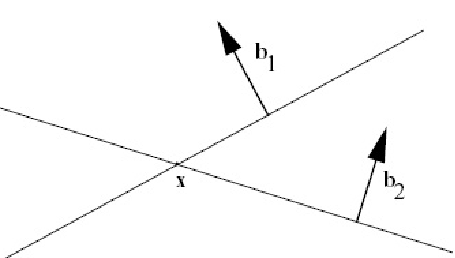
\includegraphics[height=1.5in]{2_intersection}}
\caption{Intersection of lines in 2D that are not collinear is a point.
\label{fig_intersection}}
\end{figure}

In three dimensions the equation form for describing a point will look like
\[
\matrix{
b_{1,1}x_1 &+ &b_{1,2}x_2 &+ &b_{1,3}x_3&= &c_1\cr
b_{2,1}x_1 &+ &b_{2,2}x_2 &+ &b_{2,3}x_3&= &c_2\cr
b_{3,1}x_1 &+ &b_{3,2}x_2 &+ &b_{3,3}x_3&= &c_3\cr
}
\]
where $\bb_1$, $\bb_2$ and $\bb_3$ don't all lie on the same plane. This can be
interpreted as the intersection of three planes in a single point.

Notice that going from the equation description of a point to the parametric
description just means finding the solution of the system of equations. If,
in two dimensions, the
vectors $\bb_1$ and $\bb_2$ are not collinear, or in three dimensions, 
$\bb_1$, $\bb_2$ and $\bb_3$ don't all lie on the same plane, then the system of
equations has a unique solution.

Now suppose that you are handed an arbitrary system of equations
\[
\matrix{
b_{1,1}x_1 &+ &b_{1,2}x_2 &+ &b_{1,3}x_3&= &c_1\cr
b_{2,1}x_1 &+ &b_{2,2}x_2 &+ &b_{2,3}x_3&= &c_2\cr
b_{3,1}x_1 &+ &b_{3,2}x_2 &+ &b_{3,3}x_3&= &c_3\cr
}
\]
What does the set of solutions $\xx=[x_1,x_2,x_3]$ look like?
As we just have seen, if $\bb_1$, $\bb_2$ and $\bb_3$ don't all lie on the same
plane, there is a unique solution given as the intersection of three planes.
Recall that the determinant can be used to test
whether the vectors $\bb_1$, $\bb_2$ and $\bb_3$ lie on the same plane. So a 
unique solution exists to the equation precisely when
\[
\det\left[\matrix{ b_{1,1}&b_{1,2}&b_{1,3}\cr
			b_{2,1}&b_{2,2}&b_{2,3}\cr
			b_{3,1}&b_{3,2}&b_{3,3}\cr}\right] \ne 0
\]
What happens when the determinant is zero and three 
vectors $\bb_1$, $\bb_2$ and $\bb_3$ do lie on 
the same plane? Then it could be that the three planes intersect in a line.
In this case every point on that line is a solution of the system of equations,
and the solution set has a parametric description of the form $\xx=\qq+s\aa$.
It could also be that all three planes are the same, in which case the solution
set is the plane. In this case the solution set has a parametric description of
the form $\xx=\qq+ s_1\aa_1+s_2\aa_2$
Another possibility is that two of the planes could 
be parallel with no intersection. In this case there are no solutions at all!
Some of these possibilities are illustrated in Figure~\ref{fig_planesint}.

\begin{figure}
\centerline{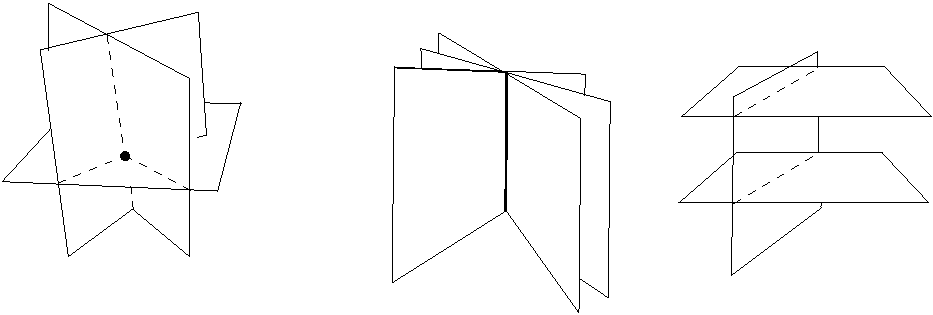
\includegraphics[height=1.5in]{2_planesint}}
\caption{Planes intersecting. \label{fig_planesint}}
\end{figure}

\begin{example} Determine whether the following system of linear equations has a solution. It is not 
necessary to find the solution or solutions if there are any. 
\[
\matrix{
x_1 &+ &x_2 &+ & x_3&= & 3 \cr
x_1 &+ &  &+ &2 x_3&= & 3 \cr
x_1 &+ &2 x_2 &+ &x_3&= & 4\cr
}
\]
{\rm We compute the determinant 
\[
\det\left[\matrix{ 1 & 1 & 1 \cr
			1 & 0 & 2 \cr
			1 & 2 & 1 \cr}\right] = -1 \ne 0
\]
Since the determinant is not zero, we know there is a unique solution point. By inspection, we can see that 
(1,1,1) solves all three equations and since we know this solution is unique, it is the only point that satisfies all three equations. In Chapter~\ref{ch:ch3} we will learn a systematic way to find the solution or all solutions (if any) of any linear systems. 
}
\end{example}

\begin{example} Determine whether the following system of linear equations has a solution. It is not 
necessary to find the solution or solutions if there are any. 
\[
\matrix{
x_1 &+ &x_2 &+ & x_3&= & 1 \cr
x_1 &+ &  &+ &x_3&= & 2 \cr
x_1 &+ &2 x_2 &+ &x_3&= & 1 \cr
}
\]
{\rm We compute the determinant 
\[
\det\left[\matrix{ 1 & 1 & 1 \cr
			1 & 0 & 1 \cr
			1 & 2 & 1 \cr}\right] = 0.
\]
Now we know that the system does not have a unique solution. Consider 
Figure~\ref{fig_planesint}. It can be made rigorous that there are two cases that could come from this system: either the solution describes a line (middle picture, infinite solutions) or the three planes do not intersect (right picture, no solutions). In Chapter~\ref{ch:ch3} we will develop an algorithm to decide this question. Here, we can look at combinations of the equations. Take twice the first equation and subtract the second to get 
\[
x_1 + 2x_2 +x_3 = 0.
\]
Since this contradicts the third equation, we see that this system has no solutions. 
}
\end{example}


\subsection{Describing the whole plane in two dimensions and all of 
space in three dimensions}

If the set we are trying to describe is the whole plane in two dimensions
or all of space in three dimensions,
then we don't need any equations, since there are no restrictions on the
points. However it does make sense to think about the parametric form. 

Lets start with two dimensions. Consider Figure~\ref{fig_basis}. 
If we pick any two vectors $\aa_1$ and $\aa_2$ that don't lie on the same line 
(that is they are different directions, not collinear),
then any vector $\xx=[x_1,x_2]$ in the plane can be 
written as $s_1\aa_1 + s_2\aa_2$. Notice that every choice of $s_1$ and $s_2$
corresponds to exactly one vector $\xx$. 
In this situation we could use the parameters
$s_1$ and
$s_2$ as co-ordinates instead of $x_1$ and $x_2$. In fact if $\aa_1$ and $\aa_2$
are unit vectors orthogonal to each other, this just amounts to changing the 
co-ordinate axes to lie along $\aa_1$ and $\aa_2$. The new co-ordinates
$[s_1,s_2]$ are then just what we were calling $[x'_1,x'_2]$ before. In fact,
even if the vectors $\aa_1$ and $\aa_2$
are not unit vectors orthogonal to each other, we can still think of them of 
lying along new co-ordinate axes. However, now the axes have been stretched and
sheared instead of just rotated, and need not lie at right angles any more. The discussion 
above motivates two important definitions. 

\begin{definition} 
A combination of vectors of the form 
\[
s_1\aa_1 + s_2\aa_2
\]
is called a {\rm linear combination} of $\{ \aa_1, \aa_2 \}$. The definition includes underlying sets of more vectors. That is, 
\[
s_1\aa_1 + s_2\aa_2 + s_3 \aa_3 
\]
is a linear combination of $\{ \aa_1, \aa_2, \aa_3 \}$ and so on. 
\end{definition} 
Writing vectors as linear combinations of a set of vectors has the interpretation of expressing the vector in a new coordinate system. 

\begin{definition} 
The set of all linear combinations of a set of vectors is called the {\rm span} of the set of vectors. 
\end{definition}

\begin{figure}
\centerline{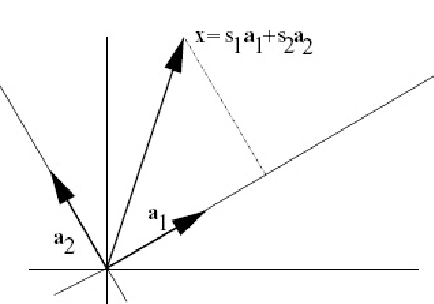
\includegraphics[height=1.5in]{2_basis}}
\caption{A basis in 2D \label{fig_basis}}
\end{figure}

The situation in three dimensions is similar. Now we must pick three vectors
$\aa_1$, $\aa_2$ and $\aa_3$ that don't lie on the same plane. Then every
vector
$\xx$ has a unique representation $\xx=s_1\aa_1+s_2\aa_2+s_3\aa_3$. We can say that the 
span of $\{ \aa_1, \aa_2, \aa_3 \}$ is all of $\mathbb{R}^3$. Again,
we could use $s_1$, $s_2$ and $s_3$ as co-ordinates in place of $x_1$, $x_2$ and
$x_3$. Again, if $\aa_1$, $\aa_2$ and $\aa_3$ are orthogonal with unit length,
then this amounts to choosing new (orthogonal) co-ordinate axes. 

\subsection{Linear dependence and independence}
\label{s:independence}

The condition in two dimensions that two vectors are not co-linear, and the 
condition in three dimensions that three vectors do not lie on the same plane
has now come up several times --- in ensuring that a system of equations has a
unique solutions and in ensuring that every vector can be written in a unique
way as a linear combination of those vectors. This condition can be tested by
computing a determinant.

We will now give this condition a name and define the analogous condition in
any number of dimensions.
Recall the definition that if $\aa_1, \aa_2, \ldots \aa_n$ is a collection of
vectors then a vector of the form 
\[
s_1\aa_1 + s_2\aa_2 + \cdots s_n\aa_n
\]
for
some choice of numbers $s_1, \ldots s_n$ is called a
{\it linear combination} of $\aa_1, \aa_2, \ldots \aa_n$.

\begin{definition}
A collection of vectors $\aa_1, \aa_2, \ldots \aa_n$ 
is called {\em linearly dependent} if some linear combination of them equals
zero, i.e., 
\[
s_1\aa_1 + s_2\aa_2 + \cdots s_n\aa_n =\zv
\]
for $s_1,\ldots s_n$ not all zero. A collection of vectors is said to be {\rm
linearly independent} if it is not linearly dependent. In other words, the
vectors $\aa_1, \aa_2, \ldots \aa_n$ are linearly independent if the only way a
linear combination of them $s_1\aa_1 + s_2\aa_2 + \cdots s_n\aa_n$ 
can equal zero is for $s_1=s_2=\cdots =s_n=0$.
\end{definition}

What does linear dependence mean in three dimensions? Suppose that $\aa_1$,
$\aa_2$ and $\aa_3$ are linearly dependent. Then there are some numbers
$s_1$, $s_2$ and $s_3$, not all zero, such that 
\[
s_1\aa_1 + s_2\aa_2 + s_3\aa_3=\zv.
\]
Suppose that $s_1$ is one of the non-zero numbers. Then we can
divide by $-s_1$ and find that 
$$-\aa_1+s_2'\aa_2 + s_3'\aa_3 =\zv$$ 
for
$s_2'=-s_2/s_1$ and $s_3'=-s_3/s_1$. Thus 
\[
\aa_1 = s_2'\aa_2 + s_3'\aa_3,
\]
or $\aa_1$ is a linear combination of $\aa_2$ and $\aa_3$. But this implies that
$\aa_1$ lies on the plane spanned by $\aa_2$ and $\aa_3$, i.e., the vectors
all lie on the same plane.  If $s_1$ happens to be 
zero we can repeat the same argument with one of the $s_i$'s which is not zero.
Thus linear dependence implies that all three vectors lie on the same plane. 
Conversely, if all three vectors lie on the same plane, then we can write one
vector as a linear combination of the other two, $\aa_1 = s_2'\aa_2 + s_3'\aa_3$
which implies $-\aa_1+s_2'\aa_2 + s_3'\aa_3 =\zv$ which says that the vectors
are linearly dependent. 

So in three dimensions, linear dependence means the vectors lie on the same
plane. 
Similarly, in two dimensions, linear dependence means the vectors are co-linear.

\begin{definition}
A collection of $n$ linearly independent 
vectors  $\aa_1, \aa_2, \ldots \aa_n$ in $\mathbb{R}^n$ dimensional space is called a
{\em basis}. 
If $\aa_1, \aa_2, \ldots \aa_n$ is a basis, then every vector 
$\xx$
can
be written in a unique way as a linear combination
\[
\xx=s_1\aa_1 + s_2\aa_2 + \cdots s_n\aa_n
\]
\end{definition} 

Two linearly independent vectors in 2D is a basis for $\mathbb{R}^2$. Three linearly independent vectors in 3D is a basis for $\mathbb{R}^3$. The span of two linearly independent vectors in $\mathbb{R}^3$ is a plane through the origin. This motivates the following:
\begin{definition}
The {\em dimension} of a span of a set $\cal C$ of linearly independent vectors is equal to the number of vectors in $\cal C$. 
\end{definition} 

\begin{example} Show that $(1,1)$ and $(2,0)$ are linearly independent. 
{\rm If they were linearly dependent by the definition they would be multiples of one another, which they are not. Thus, the vectors are linearly independent.  
}
\end{example} 

\begin{example} Write $(3,4)$ as a linear combination of $(1,1)$ and $(2,0)$.
{\rm From the previous example, we know that $(1,1)$ and $(2,0)$ are linearly independent, and so are a 
basis for $\mathbb{R}^2$ and so any vector in $\mathbb{R}^2$ can be written uniquely as a linear combination of them. We write 
\[
(3,4) = s(1,1) + t(2,0)
\]
or 
\begin{eqnarray*}
s + 2t & = & 3 \\
s + 0t & = & 4 
\end{eqnarray*}
It can be seen that writing a vector as a linear combination results in a linear system of equations. We will 
come back to this in Chapter~\ref{ch:ch3}. 
From the second component (second equation above), we see that $s=4$. Going to the first equation we can 
then determine $t= -1/2$. Thus 
\[
(3,4) = 4(1,1) -\frac{1}{2} (2,0)
\] 
}
\end{example} 

\begin{example} Show that $\{ (1,1,1), (1,1,2), (1,2,1) \}$ is a linearly independent set of vectors. 
{\rm We compute 
\[
\det\left[\matrix{ 1 & 1 & 1 \cr
			1 & 1& 2 \cr
			1 & 2 & 1 \cr}\right] = -1.
\]
Thus, the set of vectors is linearly independent. 
}
\end{example} 

\begin{example}
What is the dimension of the span of ${\cal C} = \{ (1,2,3,0), (1,1,1,1) \}$? 
{\rm By the definition of linear independence, two vectors can only be linearly dependent if they are multiples of each other. Thus, $\cal C$ is a linearly independent set and its span is two dimensional. It is a two dimensional set that includes the origin in $\mathbb{R}^4$. 
}
\end{example} 

\subsection{Problems}
%&&&

\begin{problem}
\label{op1_37}
Is the collection of vectors $\aa_1=[1,1]$, $\aa_2=[1,0]$ a basis for two
dimensional space? If so, express the vector $\xx=[0,1]$ as a linear combination
of $\aa_1$ and $\aa_2$
\end{problem}

\begin{problem}
\label{2008_a3_2} Let $\aa = [2,2,2]$ and $\bb = [3,4,1]$. Find
all vectors $\cc$ such that the list of vectors $\aa, \bb, \cc$ is 
{\em not} a basis of $\mathbb{R}^3$. 
\end{problem}

\begin{problem}
\label{2008_a3_1} Show that the collection of vectors $\aa = [1,1,1]$,
$\bb =[1,1,0]$ and $\cc = [1,0,0]$ is a basis of $\mathbb{R}^3$. Express 
$[1,2,3]$ as a linear combination of the vectors $\aa$, $\bb$ and $\cc$. 
\end{problem}

\begin{problem}
\label{2009_a3_1}
Let  the vectors ${\bf a} = [1,0,4]$, ${\bf b} = [2,-1,0] $and ${\bf c} = [8,-3,8]$. Do these vectors form a basis of $\mathbb{R}^3$? 
\end{problem}

\begin{problem}
\label{op1_38}
Is it possible for four vectors to be linearly independent in
three dimensional space?
\end{problem}

\begin{problem}
\label{2009_a3_2}
Show that the collection of vectors ${\bf a} = [2,1,3]$, ${\bf b} = [1,0,2] $ and ${\bf c} = [3,0,0]$ is a basis of $\mathbb{R}^3$. Express $[12, 2,4]$ as a linear combination of the vectors ${\bf a}, {\bf b}$ and ${\bf c}$.
\end{problem}

\begin{problem}
\label{op1_39}
Suppose that $\aa_1, \aa_2, \ldots \aa_n$ is a basis. Show that if some vector
$\xx$ has  representation $\xx=s_1\aa_1 + s_2\aa_2 + \cdots s_n\aa_n$
and $\xx=t_1\aa_1 + t_2\aa_2 + \cdots t_n\aa_n$, then $s_1=t_1$,
$s_2=t_2$,$\ldots$,$s_n=t_n$. (Hint: subtract the two expressions for $\xx$ and
use the fact that the basis vectors are linearly independent.)
\end{problem}

\begin{problem}
\label{matlab_op1_39}
(Matlab) Start by convincing yourself that the vectors $(1,3)$, and $(5,2)$ are linearly independent. This can easily be shown by writing a script that plots the vectors:
\begin{verbatim}
plot([1,0],[3,0])
hold on
plot([5,0],[2,0])
\end{verbatim}
We can extend this script by also plotting a linear combination of the two vectors:
\begin{verbatim}
alfa=1;
beta=1;
clf()
plot([alfa*1,0],[alfa*3,0])
hold on
plot([beta*5,0],[beta*2,0])
plot([alfa*1+beta*5,alfa*1],[alfa*3+beta*2,alfa*3],'--')
\end{verbatim}
Play around with the script and find parameters {\tt alfa} and {\tt beta} so that the vector $(1,1)$ can be written as a linear combination of $(1,3)$ and $(5,2)$.

\end{problem}

\section{Additional Topics}

These topics are not covered in the current version of Math 152 at UBC.

\subsection{Application: rotational motion}

Consider a rigid body rotating about an axis given by the unit vector
$\aa$ at a rate of $\Omega$ radians per second. Let $\rr$ be the
position vector of a point on the body as shown in Figure~\ref{fig_rotmot}.

\begin{figure}
\centerline{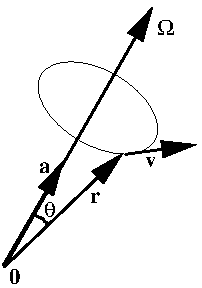
\includegraphics[height=2in]{2_rotmot}}
\caption{Rotational Motion. \label{fig_rotmot}}
\end{figure}

What is the velocity of the point? The point travels on a
circle with radius $\|\rr\|\sin(\theta)$, where $\theta$ is the angle that
$\rr$ makes with the axis. Therefore, in one second, the point travels a 
distance of $\Omega\|\rr\|\sin(\theta)$. Thus
{\begin{enumerate}
\renewcommand{\labelenumi}{(\roman{enumi})}
\item the magnitude of the velocity
is $\|{\bf v}\| = \Omega\|\rr\|\sin(\theta)$.
\item Now notice that ${\bf v}$ is
orthogonal to the plane spanned by $\aa$ and $\rr$.
\item Finally notice that $\Omega\aa$, $\rr$ and $\vv$ obey the right
hand rule.
\end{enumerate}}
The facts (i), (ii) and (iii) imply that $\vv$ is exactly the cross
product of $\Omega\aa$ and $\rr$. It is customary to let $\bf\Omega$
denote the vector $\Omega\aa$. Then
\[
{\bf v} = {\bf\Omega}\times\rr.
\]

\begin{problem}
\label{op1_19}
A body rotates at an angular velocity of $10$ rad/sec about the axis
through the points $[1,1,-1]$ and $[2,-3,1]$.  Find the velocity of
the point $[1,2,3]$ on the body.
\end{problem}

\begin{problem}
\label{2009_a2_2}
The line $L$ passing through the origin and the point
[1,1,1] passes through the midpoint of a thin metal rod of length
2 that is oriented in the direction [1,0,0]. The rod begins rotating
about $L$ at 3 revolutions per minute. What is the fastest speed
(length of velocity vector) of any point on the rod?
\end{problem}

\begin{problem}
\label{op1_20}
Imagine a plate that lies in the $xy$--plane and is rotating about the
$z$--axis. Let $P$ be a point that is painted on this plane. Denote by
$r$ the distance from $P$ to the origin, by $\theta(t)$ the angle at
time $t$ between the line from the origin to $P$ and the $x$--axis and
by $[x(t),y(t)]$ the co-ordinates of $P$ at the time $t$. Find $x(t)$
and $y(t)$ in terms of $\theta(t)$. Compute the velocity of $P$ in two
ways: 1. by differentiating $[x(t),y(t)]$ and 2. by computing
${\bf\Omega}\times\rr$.
\end{problem}

\subsection{Application: 3-D graphics}

How can we represent a three dimensional object on piece of paper or 
computer screen? Imagine the object in space and, a certain distance away,
a point $\pp$ representing the eye of the observer.
Between the observer and the object is a plane called the view plane.
The position of the origin of this plane is described by a point $\qq$, and its
orientation is given by three orthogonal unit vectors of length $1$, denoted
$\eee_1$, $\eee_2$ and $\eee_3$. (These are not the same as the standard basis
vectors $\ii$, $\jj$ and $\kk$ in this problem.) This situation is shown 
in Figure~\ref{fig_persp}. As usual, only the heads of the vectors 
(points) $\pp$, $\xx$, $\yy$ and $\qq$ are shown on the diagram. (The origin,
where the tails of these vectors lie, is not depicted at all.)
We will assume that the view plane is a distance one from the observer in the direction $\eee_3$.
Thus, $\eee_3$ can be thought of as the direction that the observer is looking.
Think of light rays leaving the object at point $\xx$ and travelling to the observer's eye
at $\pp$. At some point $\yy$ this line intersects the view plane. All the vectors $\yy$ on
the view plane that correspond to some vector $\xx$ on our object will furnish the two
dimensional representation of the object.

\begin{figure}
\centerline{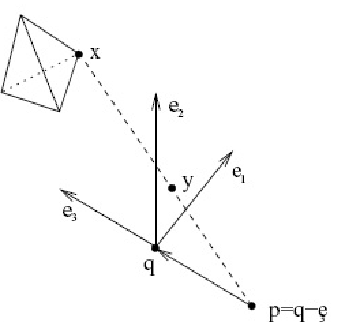
\includegraphics[height=2in]{2_persp}}
\caption{Perspective in 3-D graphics application. \label{fig_persp}}
\end{figure}

How do we determine the point $\yy$? The parametric
form of points on the plane is $\qq+s_1\eee_1+s_2\eee_2$. So we must have that
$\yy=\qq+s_1\eee_1+s_2\eee_2$ for some values of $s_1$ and $s_2$. We also know that
the vector $\xx-\pp$ is in the same direction as $\yy-\pp$. Therefore they must
be multiples, i.e., $\yy-\pp=\lambda(\xx-\pp)$ for some number $\lambda$.
Substituting in our expression for $\yy$ yields
\[
\qq+s_1\eee_1+s_2\eee_2-\pp=\lambda(\xx-\pp).
\]
Since $\qq-\pp=\eee_3$ this gives
\[
\eee_3+s_1\eee_1+s_2\eee_2=\lambda(\xx-\pp).
\]
Let us take the dot product of both sides of this equation with the unit vectors
$\eee_3$, $\eee_1$ and $\eee_2$. We can use the fact that $\eee_i\cdot\eee_j$ is zero
if $i\ne j$ and $1$ if $i=j$. Start with $\eee_3$. This gives
\[
\eee_3\cdot\eee_3 = 1 = \lambda\eee_3\cdot(\xx-\pp).
\]
This determines $\lambda$.
\[
\lambda = {{1}\over{\eee_3\cdot(\xx-\pp)}}.
\]
Now take the dot product with $\eee_1$. This gives
\[
s_1 = \lambda\eee_1\cdot(\xx-\pp) = {{\eee_1\cdot(\xx-\pp)}\over{\eee_3\cdot(\xx-\pp)}}
\]
Similarly, taking the dot product with $\eee_2$ leads to
\[
s_2= {{\eee_2\cdot(\xx-\pp)}\over{\eee_3\cdot(\xx-\pp)}}
\]

To plot the image of an object, we now simply plot the co-ordinates $s_1$ and
$s_2$  corresponding to all the points on the object on the $s_1$--$s_2$ plane.

\begin{example} Take $\pp=[11,0,0]$, $\qq=[10,0,0]$, $\eee_1=[0,1,0]$,
$\eee_2=[0,0,1]$ and $\eee_3=[-1,0,0]$. 
What is the image of the point $\xx=[1,1,1]$? 
{\rm 
We compute $\xx-\pp=[-10,1,1]$ so that
\begin{eqnarray*}
\eee_1\cdot(\xx-\pp) & = & 1 \\
\eee_2\cdot(\xx-\pp) &= & 1 \\
\eee_3\cdot(\xx-\pp) &= & 10
\end{eqnarray*}
So $s_1= s_2= 1/10$.}
\end{example}

\begin{example} Continue the previous example and 
compute the image of a line segment
between $[1,1,1]$ and $[2,0,1]$. {\rm 
These are all points of the form $\xx=[1,1,1]+
t([2,0,1]-[1,1,1]) = [1+t,1-t,1]$ as $t$ varies between $0$ and $1$.
This time we have $\xx-\pp=[1+t-11,1-t,1]$ so that
\begin{eqnarray*}
\eee_1\cdot(\xx-\pp) &= & 1-t \\
\eee_2\cdot(\xx-\pp) &= & 1 \\
\eee_3\cdot(\xx-\pp) &= & 10-t
\end{eqnarray*}
Thus $s_1 = (1-t)/(10-t)$ and $s_2=1/(10-t)$. Even though it is not immediately obvious,
the points $[s_1,s_2]$, as $t$ varies, all lie on a line segment. In fact 
\[
s_1 + 9 s_2 = (1-t)/(10-t)+9/(10-t) = (10-t)/(10-t) = 1.
\]
This shows that the points $[s_1,s_2]$ lie on a line perpendicular to $[1,9]$.}
\end{example}

In fact, it is possible to show that any line segment in space maps to a line
segment on the $s1$--$s2$ plane. Thus, to plot the image of an object consisting
of straight line segments (such as the tetrahedron in the picture) it is only
necessary to plot the vertices and then join them by straight lines.

\begin{problem}
\label{op1_33}
What are the $s_1$ and $s_2$ co=ordinates of the point $\xx=[1,2,3]$, if $\pp$,
$\qq$ are as above, $\eee_1=[0,1/\sqrt{2},1/\sqrt{2}]$ and 
$\eee_2=[0,-1/\sqrt{2},1/\sqrt{2}]$.
\end{problem}

\begin{problem}
\label{op1_34}
Plot the image on the $s_1$--$s_2$ plane of the tetrahedron whose 
vertices are located at
$[0,0,0]$, $[0,1,0]$, $[0,1/2,\sqrt{3}/2]$ and $[\sqrt{3}/6,\sqrt{6}/3,1/2]$
(Use the same values as before: $\pp=[-10,0,0]$, $\qq=[10,0,0]$, $\eee_1=[0,1,0]$,
$\eee_2=[0,0,1]$ and $\eee_3=[-1,0,0]$.)
\end{problem}

\begin{problem}
\label{op1_35}
Suppose that that points $\xx$ lie on the line $\xx=\xx_0 + t\vv$. 
Show that corresponding planar points $[s_1,s_2]$ also lie on a line. (Hint: show that
there are numbers $a$, $b$, $c$ that do not depend on $t$, so that $a s_1 + b s_2 = c$ for
every $t$.)
\end{problem}

\begin{problem}
\label{op1_36}
Consider a different drawing procedure where the point $\xx$ maps to the 
point on the view plane given by the intersection of the plane with the line
through $\xx$ parallel to $\eee_3$. Find a formula for the $s_1$ and $s_2$
co-ordinates of $\xx$.
\end{problem}

\section{Solutions to Chapter Problems}

%%%%%%%%%%%%%%%%%%%%%%%%%%%%%%%%%%%%%%%%%%%%%%%%%%%%%%%%%%%%%%%%%%%%%%%%%%%%%%%%
\noindent {\bf Solution \ref{2009_a1_1}} See Figure~\ref{2009_a1_1_sol}.

\begin{figure}[htb]
\centerline{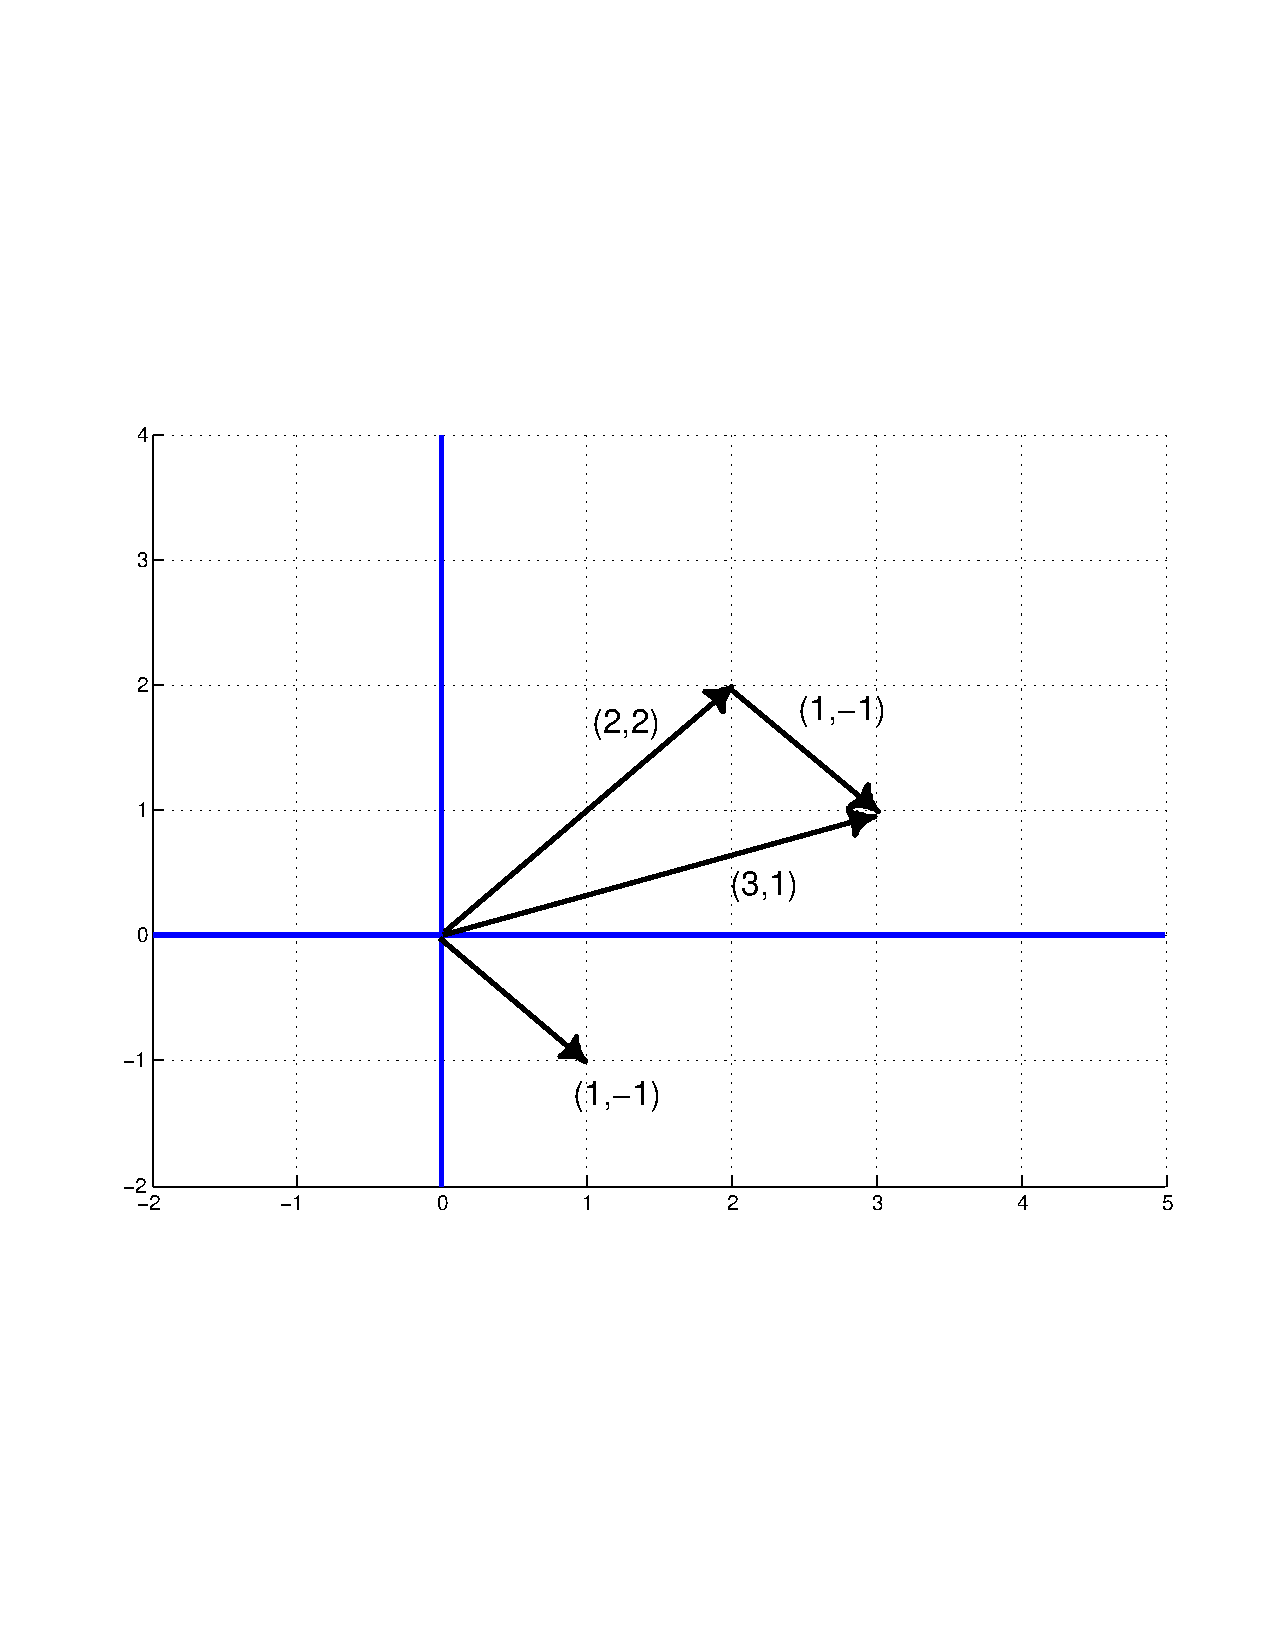
\includegraphics[height=3in]{2_2009_a1_1}}
\caption{Solution to problem \ref{2009_a1_1} \label{2009_a1_1_sol}}
\end{figure}

%%%%%%%%%%%%%%%%%%%%%%%%%%%%%%%%%%%%%%%%%%%%%%%%%%%%%%%%%%%%%%%%%%%%%%%%%%%%%%%%
\vspace{2mm}
\noindent {\bf Solution \ref{op1_1}}
{\begin{enumerate}
\renewcommand{\labelenumi}{(\roman{enumi})}
\item A straight line passing through the origin in the direction of $\aa$.
\item A ray (half line) passing through the origin in the direction of 
$\aa$.
\item A straight line parallel to $\aa$ passing through $\bb$.
\item If $\aa$ and $\bb$ do not lie on the same line:
a plane passing
through the origin parallel to $\aa$ and
$\bb$ (in two dimensions, this is the whole plane). 
If $\aa$ and $\bb$ lie on the same line: a
straight line passing through the origin in the direction of $\aa$ (and $\bb$).\par
\item If $\aa$ and $\bb$
both lie on the same line: a line passing through  $\cc$ parallel to
$\aa$ (and
$\bb$).  If $\aa$ and $\bb$ do not lie on the same line:
a plane passing
through $\cc$ parallel to $\aa$ and
$\bb$ (in two dimensions, this is the whole plane).
\end{enumerate}}

%%%%%%%%%%%%%%%%%%%%%%%%%%%%%%%%%%%%%%%%%%%%%%%%%%%%%%%%%%%%%%%%%%%%%%%%%%%%%%%%
\vspace{2mm}
\noindent {\bf Solution \ref{op1_2}}
$\aa-\bb$ is the vector that when added to $\bb$ gives $\aa$. So if we draw it
with its tail at $\bb$ then its head is at $\aa$. Similarly $\bb - \aa$ when
drawn with its tail at $\aa$ has its head at $\bb$.

%%%%%%%%%%%%%%%%%%%%%%%%%%%%%%%%%%%%%%%%%%%%%%%%%%%%%%%%%%%%%%%%%%%%%%%%%%%%%%%%

\vspace{2mm}
\noindent {\bf Solution \ref{op1_3}}
To find the midpoint we add half of the vector with its tail at $\aa$ and head
at $\bb$ to $\aa$. So the midpoint is $\aa + (1/2)(\bb-\aa)= (1/2)(\aa+\bb)$.
Similarly, the point one third of the way from $\aa$ to $\bb$ is
$\aa + (1/3)(\bb-\aa) = (2/3)\aa + (1/3)\bb$. 

%%%%%%%%%%%%%%%%%%%%%%%%%%%%%%%%%%%%%%%%%%%%%%%%%%%%%%%%%%%%%%%%%%%%%%%%%%%%%%%%
\vspace{2mm}
\noindent {\bf Solution \ref{op1_4}}
The line segment is given by the vectors $\aa + t(\bb-\aa)$ as $t$ varies
between $0$ and $1$.

%%%%%%%%%%%%%%%%%%%%%%%%%%%%%%%%%%%%%%%%%%%%%%%%%%%%%%%%%%%%%%%%%%%%%%%%%%%%%%%%
\vspace{2mm}
\noindent {\bf Solution \ref{2009_a1_2}}
$\aa = (1,2);\qquad \bb = (1,-2)$
{\begin{enumerate}
\renewcommand{\labelenumi}{(\alph{enumi})}
\item $\aa + \bb = (2,0)$
\item $2 \aa = (2,4)$
\item $\aa - \bb = (0,4)$
\item $\aa \cdot \bb = 1-4 = -3$.
\item $\| \bb \| = \sqrt{1 + 4} = \sqrt{5}$.
\end{enumerate}}

%%%%%%%%%%%%%%%%%%%%%%%%%%%%%%%%%%%%%%%%%%%%%%%%%%%%%%%%%%%%%%%%%%%%%%%%%%%%%%%%
\vspace{2mm}
\noindent {\bf Solution \ref{2008_a1_3}}
The radius of the circle is 
\[
\| (2,5) - (3,3) \| = \|(-1,2)\| = \sqrt{1+4} = \sqrt{5}.
\]
Thus using the standard equation for a circle 
\[
(x-2)^2 + (y-5)^2 = (\sqrt{5})^2 = 5.
\]

%%%%%%%%%%%%%%%%%%%%%%%%%%%%%%%%%%%%%%%%%%%%%%%%%%%%%%%%%%%%%%%%%%%%%%%%%%%%%%%%
\vspace{2mm}
\noindent {\bf Solution \ref{op1_5}}
The equation is $\|\xx-\aa\| = r$, or
\[
\sqrt{(x_1-a_1)^2+(x_2-a_2)^2+(x_3-a_3)^2} = r
\]
or
\[
(x_1-a_1)^2+(x_2-a_2)^2+(x_3-a_3)^2 = r^2
\]

%%%%%%%%%%%%%%%%%%%%%%%%%%%%%%%%%%%%%%%%%%%%%%%%%%%%%%%%%%%%%%%%%%%%%%%%%%%%%%%
\vspace{2mm}
\noindent {\bf Solution \ref{op1_6}}
The midpoint of the sphere is the midpoint of $[2,1,4]$ and $[4,3,10]$,
i.e., $(1/2)([2,1,4]+[4,3,10]) = [3,2,7]$. The radius is half the distance
between $[2,1,4]$ and $[4,3,10]$, i.e., \par $(1/2)\sqrt{(2-4)^2+(1-3)2+(4-10)^2} =
\sqrt{11}$. Thus the equation is
\[
(x_1-3)^2+(x_2-2)^2+(x_3-7)^2 = 11.
\]

%%%%%%%%%%%%%%%%%%%%%%%%%%%%%%%%%%%%%%%%%%%%%%%%%%%%%%%%%%%%%%%%%%%%%%%%%%%%%%%%
\vspace{2mm}
\noindent {\bf Solution \ref{op1_7}}
{\begin{enumerate}
\renewcommand{\labelenumi}{(\alph{enumi})}
\item $\aa\cdot\bb=-2+6=4$, $\theta = \arccos(4/(\sqrt{5}\sqrt{13})) =
1.05\ldots$
\item $\aa\cdot\bb= 1$, $\theta = 1.249\ldots$
\item $\aa\cdot\bb= 4$, $\theta = 0$
\item $\aa\cdot\bb= 2$, $\theta = 1.079\ldots\ldots$
\item $\aa\cdot\bb= 0$, $\theta = \pi/2\ldots$
\end{enumerate}}

%%%%%%%%%%%%%%%%%%%%%%%%%%%%%%%%%%%%%%%%%%%%%%%%%%%%%%%%%%%%%%%%%%%%%%%%%%%%%%%%
\vspace{2mm}
\noindent {\bf Solution \ref{2009_a1_4}}
Consider the dot product to determine angles between vectors, not the dot product (which only applies to 3D and cannot distinguish angles $\theta$ in the range $(0,\pi/2)$ from those in $(\pi/2,\pi)$, as discussed in the solution to problem \ref{op1_7} in the online notes).

\begin{enumerate}
\renewcommand{\labelenumi}{(\alph{enumi})}
\item $\aa = (1,1,1),\qquad \bb = (3,1,-2) \\ \aa\cdot\bb = 3+1-2 = 2\\
||\aa|| = \sqrt{3},\qquad ||\bb|| = \sqrt{3^2+1^2+(-2)^2}=\sqrt{14}.\\
\cos\theta = \frac{2}{\sqrt{3}\sqrt{14}},\qquad \theta = \cos^{-1}\frac{2}{\sqrt{3}\sqrt{14}}
\simeq 1.26 $ radians, or $\simeq 72.0^o$

\item Using $\aa\cdot\bb$ and $||\aa||$ above,\\
$proj_{\aa}\bb = \frac{2}{3}(1,1,1)=\left(\frac{2}{3},\frac{2}{3},\frac{2}{3}\right).$
Remember, $proj_{\aa}\bb$ should be in the direction of $\aa$.

\end{enumerate}

%%%%%%%%%%%%%%%%%%%%%%%%%%%%%%%%%%%%%%%%%%%%%%%%%%%%%%%%%%%%%%%%%%%%%%%%%%%%%%%%
\vspace{2mm}
\noindent {\bf Solution \ref{2008_a1_5}}
\begin{eqnarray*}
\aa = (1,4,0) & & \| \aa \| = \sqrt{17} \\
\bb = (2,-1,5) & & \| \bb \| = \sqrt{4 + 1 + 25} = \sqrt{30} 
\end{eqnarray*}
{\begin{enumerate}
\renewcommand{\labelenumi}{(\alph{enumi})}
\item $\cos \theta = \frac{\bb \cdot \aa}{\| \aa \| \| \bb \|} = 
   \frac{2-4}{\sqrt{17} \sqrt{30}} = \frac{-2}{\sqrt{510}}$ so
\[
\theta = \cos^{-1} \left( \frac{-2}{\sqrt{510}} \right) \approx 1.66 
\mbox{\ \ in radians or $\approx 95^\circ$}
\]
\item $\mbox{proj}_\aa \bb = \frac{\bb \cdot \aa}{\| \aa \|^2} \aa 
   = \frac{-2}{17} (1,4,0) = (-2/17, -8/17,0)$.
\end{enumerate}}

%%%%%%%%%%%%%%%%%%%%%%%%%%%%%%%%%%%%%%%%%%%%%%%%%%%%%%%%%%%%%%%%%%%%%%%%%%%%%%%%
\vspace{2mm}
\noindent {\bf Solution \ref{op1_8}}
The dot product is zero if $-1+2+s=0$, i.e., if $s=-1$.

%%%%%%%%%%%%%%%%%%%%%%%%%%%%%%%%%%%%%%%%%%%%%%%%%%%%%%%%%%%%%%%%%%%%%%%%%%%%%%%%
\vspace{2mm}
\noindent {\bf Solution \ref{op1_9}}
Let $\aa=[1,2,3]$, $\bb=[4,0,5]$ and $\cc=[3,4,6]$. The sides of the triangle
are in the directions of $\aa-\bb=[-3,2,-2]$, $\aa-\cc=[-2,-2,-3]$,
and $\bb-\cc=[1,-4,-1]$. To see if there
are any right angles we compute
$(\aa-\bb)\cdot(\aa-\cc)=[-3,2,-2]\cdot[-2,-2,-3]=8$,
$(\aa-\bb)\cdot(\bb-\cc)=[-3,2,-2]\cdot[1,-4,-1]=-9$ and
$(\aa-\cc)\cdot(\bb-\cc)=[-2,-2,-3]\cdot[1,-4,-1]=9$.
Since none of these are zero, there are no right angles.

%%%%%%%%%%%%%%%%%%%%%%%%%%%%%%%%%%%%%%%%%%%%%%%%%%%%%%%%%%%%%%%%%%%%%%%%%%%%%%%%
\vspace{2mm}
\noindent {\bf Solution \ref{2009_a1_5}}
If $[c_1, 1, c_2] = s[2, -2, 3]$, with $s$ a scalar multiple, then $s=-\frac{1}{2}$ (from the values in the second component), hence: \\
$c_1=-1,\qquad c_2 = -3/2$.

%%%%%%%%%%%%%%%%%%%%%%%%%%%%%%%%%%%%%%%%%%%%%%%%%%%%%%%%%%%%%%%%%%%%%%%%%%%%%%%%
\vspace{2mm}
\noindent {\bf Solution \ref{op1_10}}
The problem becomes much simpler if we choose the $y$ axis to run
along the runway and the x axis to run perpendicular to the runway. Replace
the wind and plane velocities by vectors ${\bf w}$ and ${\bf p}$ as on the
diagram in Figure~\ref{fig_plane}.

\begin{figure}
\centerline{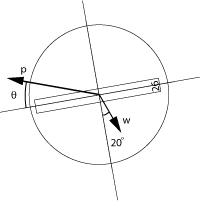
\includegraphics[height=2in]{2_plane}}
\caption{Coordinate system for Solution \ref{op1_10}. \label{fig_plane}}
\end{figure}

The wind vector has components $[-10\cos(20^\circ ), -10\sin(20^\circ )]$
while the plane velocity has components $[70\sin(\theta), 70\cos(\theta)]$.
We want the $x$ component to be zero hence we need
$10\cos(20^\circ)=70\sin(\theta)$. This gives $\theta = 7.7^\circ$, i.e,
the get the heading of the plane we have to add $7.7^\circ$ to the runway
direction. Thus the plane's heading is 267.7. The groundspeed is the magnitude
of the velocity, in this case simply the $y$ component given by
$70\cos(7.7^\circ)-10\sin(20^\circ)= 66$ knots.

%%%%%%%%%%%%%%%%%%%%%%%%%%%%%%%%%%%%%%%%%%%%%%%%%%%%%%%%%%%%%%%%%%%%%%%%%%%%%%%%
\vspace{2mm}
\noindent {\bf Solution \ref{op1_11}}
If we use the co-ordinate system where the $x$ axis is horizontal
and the $y$ axis is vertical, then the force of gravity is ${\bf F}_g=[0,-mg]$
The unit vector in the direction along the shaft is
${\bf p}=[-\sin(\theta),\cos(\theta)]$. The
force ${\bf F}_s$ exerted by the shaft is in the direction of the shaft,
hence a multiple of
${\bf p}$. So ${\bf F}_s = t{\bf p}$ for some number $t$. To find $t$ we use
that the component of the total force in the direction of the shaft must be
zero. Thus ${\rm proj}_{\bf p}{\bf F}_g +  {\bf F}_s = 0$, i.e.
${\bf p}\cdot{\bf F}_g + t=0$, i.e., $t=mg\cos(\theta)$. Thus the total force
is $ {\bf F}_g+{\bf F}_s=[0,-mg]+mg\cos(\theta)[-\sin(\theta),\cos(\theta)]
=mg[-\cos(\theta)\sin(\theta), -1+\cos^2(\theta)]$. Note that this is orthogonal
to ${\bf p}$, as it must be.

If we use co-ordinates where the $y$ axis runs along the shaft of the pendulum,
and the $x$ axis perpendicular to it, then
${\bf F}_g=[-mg\sin(\theta),-mg\cos(\theta)]$ while ${\bf F}_s=[0,t]$ for some
value of $t$. In this case it is simply the $y$ component that must be zero,
so $t=mg\cos(\theta)$ and ${\bf F}_g+{\bf F}_s=[-mg\sin(\theta),0]$

%%%%%%%%%%%%%%%%%%%%%%%%%%%%%%%%%%%%%%%%%%%%%%%%%%%%%%%%%%%%%%%%%%%%%%%%%%%%%%%%

\vspace{2mm}
\noindent {\bf Solution \ref{matlab_op1_11}}
\begin{verbatim}
sqrt(a(1)^2+a(2)^2)  
\end{verbatim}


%%%%%%%%%%%%%%%%%%%%%%%%%%%%%%%%%%%%%%%%%%%%%%%%%%%%%%%%%%%%%%%%%%%%%%%%%%%%%%%%

\vspace{2mm}
\noindent {\bf Solution \ref{op1_12}}
$[1,2,3]\times [4,5,6]=[-3,6,-3]$

%%%%%%%%%%%%%%%%%%%%%%%%%%%%%%%%%%%%%%%%%%%%%%%%%%%%%%%%%%%%%%%%%%%%%%%%%%%%%%%%
\vspace{2mm}
\noindent {\bf Solution \ref{2009_a2_1}}
\begin{eqnarray*}
\det \left[ \begin{array}{ccc}
	1& 1& 1 \\
	1& 2& 3 \\
	1& 0& -1
	    \end{array}
\right] &=& 1(-2-0) - 1(-1-3) + 1(0-2)\\
&=& -2+4-2 = 0
\end{eqnarray*}
Since the determinant is zero, the volume of the parallelepiped generated by the row vectors is zero. This implies that the vectors lie on the same plane.

%%%%%%%%%%%%%%%%%%%%%%%%%%%%%%%%%%%%%%%%%%%%%%%%%%%%%%%%%%%%%%%%%%%%%%%%%%%%%%%%
\vspace{2mm}
\noindent {\bf Solution \ref{op1_13}}
$\aa\cdot(\aa\times\bb) = [a_1, a_2, a_3]\cdot [a_2 b_3 - a_3 b_2, a_3 b_1- a_1 b_3,
a_1 b_2 - a_2 b_1] = a_1 a_2 b_3 - a_1 a_3 b_2 + a_2 a_3 b_1 - a_2 a_1 b_3
+ a_3 a_1 b_2 - a_3 a_2 b_1 = 0$. Now $\bb\cdot(\aa\times\bb) = -\bb\cdot(\bb\times\aa)
= 0$ by the previous calculation.

%%%%%%%%%%%%%%%%%%%%%%%%%%%%%%%%%%%%%%%%%%%%%%%%%%%%%%%%%%%%%%%%%%%%%%%%%%%%%%%%
\vspace{2mm}
\noindent {\bf Solution \ref{2008_a2_1}}
{\begin{enumerate}
\renewcommand{\labelenumi}{(\alph{enumi})}
\item $((1,4,-1)\cdot(2,1,3)) ((2,1,4) \times (1,4,9))$
\begin{eqnarray*}
 & = & (2+4-3) \left| \begin{array}{ccc} 
\hat{i} & \hat{j} & \hat{k} \\
2 & 1 & 4 \\
1 & 4 & 9 
\end{array} \right| \\
 & = & 3 (\hat{i} (9-16) + \hat{j}(4-18) + \hat{k}(8-1) \\
 & = & 3 (-7,-14,7) = (-21,-42,21) 
\end{eqnarray*}
\item $(7,1,0)\cdot ((2,0,-1) \times (1,4,3))$
\begin{eqnarray*}
 & = & (7,1,0) \cdot \left| \begin{array}{ccc}
\hat{i} & \hat{j} & \hat{k} \\
2 & 0 & -1 \\
1 & 4 & 3
\end{array} \right| \\
 & = & (7,1,0) \cdot (\hat{i} (0+4) + \hat{j}(-1-6) + \hat{k}(8-0) \\
 & = & (7,1,0) \cdot (4,-7,8) = 28-7+0 = 21
\end{eqnarray*}
\item $(\aa \times \bb) \times (\bb \times \aa)$
\[
= (\aa \times \bb) \times (- \aa \times \bb) = 
   - (\aa \times \bb) \times (\aa \times \bb) = {\bf 0} 
\]
because $\cc \times \cc = {\bf 0}$ for any vector $\cc$. 
\end{enumerate}}

%%%%%%%%%%%%%%%%%%%%%%%%%%%%%%%%%%%%%%%%%%%%%%%%%%%%%%%%%%%%%%%%%%%%%%%%%%%%%%%%
\vspace{2mm}
\noindent {\bf Solution \ref{op1_14}}
Here we are assuming that $\theta$ lies in $[0, \pi]$ so that $\sin(\theta)$ is
positive. The quantity $\|\aa\|$ is the length of the base of the parallelogram
while $\|\bb\|\sin(\theta)$ is the height. The area of a parallelogram is the
product of these. 

%%%%%%%%%%%%%%%%%%%%%%%%%%%%%%%%%%%%%%%%%%%%%%%%%%%%%%%%%%%%%%%%%%%%%%%%%%%%%%%%
\vspace{2mm}
\noindent {\bf Solution \ref{op1_15}}
Since $\aa\times\bb=-\bb\times\aa$ it is never true that
$\aa\times\bb=-\bb\times\aa$, unless $\aa\times\bb=\zv$. For the other example,
just try ${\bf i}$, ${\bf j}$ and ${\bf k}$. We have 
${\bf i}\times{\bf j}={\bf k}$ so 
${\bf i}\times({\bf i}\times{\bf j})={\bf i}\times {\bf k}=-{\bf j}$ On the other hand
$({\bf i}\times{\bf i})\times{\bf j}=\zv\times{\bf j}=\zv$

%%%%%%%%%%%%%%%%%%%%%%%%%%%%%%%%%%%%%%%%%%%%%%%%%%%%%%%%%%%%%%%%%%%%%%%%%%%%%%%%
\vspace{2mm}
\noindent {\bf Solution \ref{matlab_op1_15}}
\begin{verbatim}
a=rand(3,1);
b=rand(3,1);
c=rand(3,1);
cross(a,b) - cross(b,a)
cross(a,cross(b,c)) - cross(cross(a,b),c)
\end{verbatim}
This actually constitutes a proof, since we found a counter example. We don't have to show that it's always the case, we only had to show that in general the two assertions are not true.

%%%%%%%%%%%%%%%%%%%%%%%%%%%%%%%%%%%%%%%%%%%%%%%%%%%%%%%%%%%%%%%%%%%%%%%%%%%%%%%%
\vspace{2mm}
\noindent {\bf Solution \ref{op1_16}}
This a just a long calculation. One way to break it up is to consider $\aa=$ 
${\bf i}$, ${\bf j}$ and ${\bf k}$ separately. Suppose we can prove it for these
special cases. Then write a general 
$\aa$ as $a_1{\bf i}+a_2{\bf j}+a_3{\bf k}$. Then $\aa\times(\bb\times\cc)=
a_1{\bf i}\times(\bb\times\cc)+a_2{\bf j}\times(\bb\times\cc)
+a_3{\bf k}\times(\bb\times\cc)$ Assuming for the moment we know that the
special cases hold, then this equals $a_1((\ii\cdot\cc)\bb-(\ii\cdot\bb)\cc)
+a_2((\jj\cdot\cc)\bb-(\jj\cdot\bb)\cc) 
+ a_3((\kk\cdot\cc)\bb-(\kk\cdot\bb)\cc)= (\aa\cdot\cc)\bb-(\aa\cdot\bb)\cc$
Now we still have to prove the special cases. For example if $\aa=\ii$ we have
$\ii\times(\bb\times\cc) =
\det\left[\matrix{\ii&\jj&\kk\cr 1&0&0\cr
b_2c_3-b_3c_2&b_3c_1-b_1c_3&b_1c_2-b_2c_1\cr}\right]
=-(b_1c_2-b_2c_1)\jj+(b_3c_1-b_1c_3)\kk=[0,-b_1c_2+b_2c_1,b_3c_1-b_1c_3]
$ On the other
hand$(\ii\cdot\cc)\bb-(\ii\cdot\bb)\cc=c_1[b_1,b_2,b_3]-b_1[c_1,c_2,c_3]=
[0, c_1b_2-b_1c_2, c_1b_3-b_1c_3]$. The other two are similar.

%%%%%%%%%%%%%%%%%%%%%%%%%%%%%%%%%%%%%%%%%%%%%%%%%%%%%%%%%%%%%%%%%%%%%%%%%%%%%%%%
\vspace{2mm}
\noindent {\bf Solution \ref{matlab_op1_16}}
\begin{verbatim}
a=rand(3,1);
b=rand(3,1);
c=rand(3,1);
cross(a,cross(b,c)) - (dot(a,c)*b - dot(a,b)*c)
\end{verbatim}

%%%%%%%%%%%%%%%%%%%%%%%%%%%%%%%%%%%%%%%%%%%%%%%%%%%%%%%%%%%%%%%%%%%%%%%%%%%%%%%%
\vspace{2mm}
\noindent {\bf Solution \ref{op1_17}}
$(\aa\times\bb)\cdot(\cc\times\dd)=((\aa\times\bb)\times\cc)\cdot\dd$ (by
property 5) $= - (\cc\times(\aa\times\bb))\cdot\dd$ (by property 1)
$=-((\cc\cdot\bb)\aa+(\cc\cdot\aa)\bb)\cdot\dd
=-(\cc\cdot\bb)(\aa\cdot\dd)+(\cc\cdot\aa)(\bb\cdot\dd)$

%%%%%%%%%%%%%%%%%%%%%%%%%%%%%%%%%%%%%%%%%%%%%%%%%%%%%%%%%%%%%%%%%%%%%%%%%%%%%%%%
\vspace{2mm}
\noindent {\bf Solution \ref{2008_a2_5}}
{\begin{enumerate}
\renewcommand{\labelenumi}{(\alph{enumi})}
\item Let ${\bf v} = \aa \times (\aa \times \bb)$. Since $\aa \times \bb$ 
is orthogonal to the paper, $\bf v$ must lie in the plane of the paper. 
$\bf v$ is also orthogonal to $\aa$. Checking orientations with the 
right hand rule, there are only two sketches (up to rotation and resizing 
the vectors) shown in Figure~\ref{fig_newfig2}. 
\item $ \aa \times (\aa \times \bb)= 
(\bb \cdot \aa) \aa - (\aa \cdot \aa) \bb$ by property 2 in the notes. 
\[
 = \| \aa \|^2 \left( \frac{\bb \cdot \aa}{\| \aa \|^2} \aa - \bb \right) 
 = \| \aa \|^2(\mbox{proj}_\aa \bb - \bb).
\]
\end{enumerate}}

\begin{figure}
\centerline{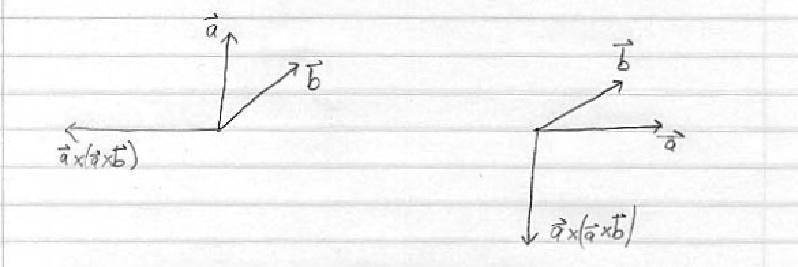
\includegraphics[height=1.5in]{2_newfig2}}
\caption{Vector sketch for the solution to \ref{2008_a2_5}.
\label{fig_newfig2}}
\end{figure}

%%%%%%%%%%%%%%%%%%%%%%%%%%%%%%%%%%%%%%%%%%%%%%%%%%%%%%%%%%%%%%%%%%%%%%%%%%%%%%%%
\vspace{2mm}
\noindent {\bf Solution \ref{op1_18}}
Actually there is no one right answer to this problem. But
in two dimensions the analog of the cross product could be an
operation on a single vector say $\times(\aa)$ with the property that
$\times(\aa)\cdot\bb=\det\left[\matrix{a_1&a_2\cr b_1&b_2\cr}\right]$ This
implies that $\times(\aa) = [a_2,-a_1]$. Note that $\times(\aa)$ is orthogonal
to $\aa$. The answer in $4$ dimensions is a little more obscure. In this case
the cross product could be an operation on three vectors 
that produces a vector that is orthogonal to all of them. One way of producing
such a vector would be to do the formal calculation of a $4\times 4$ determinant,
where the first row contains the four unit vectors $\eee_1$, $\eee_2$, $\eee_3$
and $\eee_4$, while the other three rows contain the entries of 
$\aa$,$\bb$ and $\cc$. Do you see why? 
(There is another possible, perhaps better answer, involving a different
type of product called the wedge product.)

%%%%%%%%%%%%%%%%%%%%%%%%%%%%%%%%%%%%%%%%%%%%%%%%%%%%%%%%%%%%%%%%%%%%%%%%%%%%%%%%
\vspace{2mm}
\noindent {\bf Solution \ref{op1_21}}
Let $\qq$ be a point on the line. Then the projection of $\xx$ in the direction
of $\bb$ is ${{\xx\cdot\bb}\over{\|\bb\|^2}}$. The set of all points whose
projection in the direction of $\bb$ are the same as the projection of the point
$\qq$ in the direction of $\bb$ is therefore the set of points $\xx$ such that
${{\xx\cdot\bb}\over{\|\bb\|^2}}={{\qq\cdot\bb}\over{\|\bb\|^2}}$. Multiplying
both sides by by $\|\bb\|^2$ gives $\xx\cdot\bb=\qq\cdot\bb$.

%%%%%%%%%%%%%%%%%%%%%%%%%%%%%%%%%%%%%%%%%%%%%%%%%%%%%%%%%%%%%%%%%%%%%%%%%%%%%%%%
\vspace{2mm}
\noindent {\bf Solution \ref{op1_22}}
The line is in the direction of $\aa=[7,5]-[0,1]=[7,4]$ and is therefore
perpendicular to $\bb=[4,-7]$. $\qq=[0,1]$ is a point on the line. So the
parametric form for the line is $[0,1]+s[7,4]$ and the equation form is
$4x_1-7x_2=-7$. So five points on the line are (picking $s=-2,1,0,1,2$)
$[-14,-7],[-7,-3],[0,1],[7,5],[14,9]$. To check whether $[1012/3,1069/21]$ lies
on the line, plug it into the equation: $4\cdot 1012/3-7\cdot 1069/21 \ne -7$
so the point does not lie on the line.

%%%%%%%%%%%%%%%%%%%%%%%%%%%%%%%%%%%%%%%%%%%%%%%%%%%%%%%%%%%%%%%%%%%%%%%%%%%%%%%%
\vspace{2mm}
\noindent {\bf Solution \ref{op1_23}}
We can take $\qq=[1,1]$ and $\bb=[2,1]$ so the equation is $2x_1+x_2=3$.

%%%%%%%%%%%%%%%%%%%%%%%%%%%%%%%%%%%%%%%%%%%%%%%%%%%%%%%%%%%%%%%%%%%%%%%%%%%%%%%%
\vspace{2mm}
\noindent {\bf Solution \ref{op1_24}}
We have to find a point on the line. Try for one of the form $[t,0]$. This
is on the line if $t-3\cdot 0=5$. So $[5,0]$ is on the line. The vector
orthogonal to the line is $[1,-3]$ so a vector parallel is $[3,1]$. Thus
the parametric form is $[5,0]+s[3,1]$.

%%%%%%%%%%%%%%%%%%%%%%%%%%%%%%%%%%%%%%%%%%%%%%%%%%%%%%%%%%%%%%%%%%%%%%%%%%%%%%%%
\vspace{2mm}
\noindent {\bf Solution \ref{op1_25}}
Pick a point $\qq$ on the line and let $\bb$ be orthogonal to the line. Then
the distance from a point $\xx$ to the line is the length of the
projection of $\xx-\qq$ onto $\bb$ as shown in Figure~\ref{fig_projl}.
\begin{figure}
\centerline{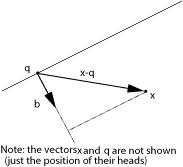
\includegraphics[height=2in]{2_projl}}
\caption{The projection used in Solution \ref{op1_25}. \label{fig_projl}}
\end{figure}
In this case we can take $\bb=[3,-4]$, $\qq=[0,1]$ and $\xx=[-2,3]$. The
projection is $((\xx-\qq)\cdot\bb/\|\bb\|^2)\bb$ This equals
$([-2,2]\cdot[3,-4]/25)[3,-4]=(-14/25)[3,4]$ The length of this vector
is $14/5$.

%%%%%%%%%%%%%%%%%%%%%%%%%%%%%%%%%%%%%%%%%%%%%%%%%%%%%%%%%%%%%%%%%%%%%%%%%%%%%%%%
\vspace{2mm}
\noindent {\bf Solution \ref{2009_a2_3}}
{\begin{enumerate}
\renewcommand{\labelenumi}{(\alph{enumi})}
\item the normal direction to the plane is $(1,-1,2)$
\item the point $(7,0,0)$ is on the plane (look for a solution with $y=z=0$ that is the intersection of the plane with the line of the x-axis).
\end{enumerate}}

%%%%%%%%%%%%%%%%%%%%%%%%%%%%%%%%%%%%%%%%%%%%%%%%%%%%%%%%%%%%%%%%%%%%%%%%%%%%%%%%
\vspace{2mm}
\noindent {\bf Solution \ref{op1_26}}
The midpoint between $\bb$ and $\cc$ is $(\bb+\cc)/2$. So the vector from
$\aa$ to this midpoint is $(\bb+\cc)/2-\aa$ and thus the parametric form for
the median is $\aa + t((\bb+\cc)/2-\aa)$. Similarly the parametric forms for the
other medians is $\bb + s((\aa+\cc)/2-\bb$ and $\cc + r((\aa+\bb)/2-\cc)$. When
$t=s=r=2/3$ these lines meet at the common point $(\aa+\bb+\cc)/3$

%%%%%%%%%%%%%%%%%%%%%%%%%%%%%%%%%%%%%%%%%%%%%%%%%%%%%%%%%%%%%%%%%%%%%%%%%%%%%%%%
\vspace{2mm}
\noindent {\bf Solution \ref{2008_a2_3}}
The line is in direction $(0,1,3)$. Two vectors which are orthogonal 
to the line are $(1,0,0)$ and $(0,3,-1)$, because $(1,0,0) \cdot (0,1,3) = 0$ 
and $(0,3,-1) \cdot (0,1,3) = 0$. Note that there are other choices for these 
two vectors that lead to different correct answers below. There will 
be two equations of the form 
\begin{eqnarray*}
x & = & c_1 \\
3y - z & = & c_2 
\end{eqnarray*}
Substituting the point $(2,0,4)$ that we know is on the line gives 
$c_1 = 2$ and $c_2 = 4$. Thus an equation form of the line is 
\begin{eqnarray*}
x & = & 2 \\
3y - z & = & 4 
\end{eqnarray*}

%%%%%%%%%%%%%%%%%%%%%%%%%%%%%%%%%%%%%%%%%%%%%%%%%%%%%%%%%%%%%%%%%%%%%%%%%%%%%%%%
\vspace{2mm}
\noindent {\bf Solution \ref{2008_a2_4}}
To find an equation for the plane we need an orthogonal vector 
\[
(0,1,-3) \times (-1,2,0)  =  \left| \begin{array}{ccc}
\hat{i} & \hat{j} & \hat{k} \\
0 & 1 & -3 \\
-1 & 2 & 0
\end{array} \right| = \hat{i} (0+6) + \hat{j} (3-0) + \hat{k}(0+1)
   = (6,3,1).
\]
So an equation for the plane is $6x + 3y + z = c$ and we know that 
$c=0$ since the plane goes through the origin. Any point on the line has the 
form 
\[
(2,-1,6) + s(1,-1,0) = (2+s, -1-s,6).
\]
Substituting this into the equation for the plane gives
\begin{eqnarray*}
6 (2+s) + 3(-1-s) + 6 & = & 0 \\
3s + 15 & = & 0 \\
s & = & -5 
\end{eqnarray*}
So the intersection point is 
\[
(2,-1,6) - 5(1,-1,0) = (2,-1,6)+(-5,5,0) = (-3,4,6). 
\]
{\em Note:} it can be checked that $t=-2$ and $u=3$ in the parametric form 
of the plane gives this point as well.

%%%%%%%%%%%%%%%%%%%%%%%%%%%%%%%%%%%%%%%%%%%%%%%%%%%%%%%%%%%%%%%%%%%%%%%%%%%%%%%%
\vspace{2mm}
\noindent {\bf Solution \ref{2009_a2_4}}
Points on the line satisfy
\begin{eqnarray*}
x &=& 1+t\\
y &=& 2\\
z &=& 3-t.
\end{eqnarray*}

To be on the plane, $x+2y-z=5$, or $(1+t) + 2(2) - (3-t) = 5$, or $2t+2=5$, or $t=3/2$.

Thus the intersection occurs at $(1,2,3) + (\frac{3}{2})(1,0,-1) = (\frac{5}{2},2,\frac{3}{2})$.

%%%%%%%%%%%%%%%%%%%%%%%%%%%%%%%%%%%%%%%%%%%%%%%%%%%%%%%%%%%%%%%%%%%%%%%%%%%%%%%%
\vspace{2mm}
\noindent {\bf Solution \ref{op1_27}}
Two vectors in the direction of the plane are $[1,1,0]-[1,0,1]=[0,1,-1]$ and
$[0,1,1]-[1,0,1]=[-1,1,0]$ To find a normal vector take the cross product
$[0,1,-1]\times[-1,1,0]=[1,1,1]$. So the equation of the plane is
$x_1+x_2+x_3=2$.

%%%%%%%%%%%%%%%%%%%%%%%%%%%%%%%%%%%%%%%%%%%%%%%%%%%%%%%%%%%%%%%%%%%%%%%%%%%%%%%%
\vspace{2mm}
\noindent {\bf Solution \ref{op1_28}}
The centre of the sphere lies in the plane halfway between the planes
$x_1+x_2+x_3=3$ and $x_1+x_2+x_3=9$. This is the plane $x_1+x_2+x_3=6$.
So the centre satisfies the three equations
\[
\matrix{
x_1     &+      x_2     &+      x_3     &=      6\cr
2x_1    &-      3x_2    &       &=      0\cr
3x_1    &       &-      x_3     &=      0\cr
}
\]
We will develop efficient techniques for solving such systems of equations.
For now, we can just use brute force: The second equation says $x_2=2x_1$ and
the third $x_3=3x_1$. Substituting this into the first equation yields$ x_1=1$,
so $x_2=2$ and $x_3=3$. Therefore the centre of the sphere is $[1,2,3]$. To
compute the radius, we must find the distance between the planes
$x_1+x_2+x_3=3$ and $x_1+x_2+x_3=6$ If we divide the equations by
$\|[1,1,1]\|=\sqrt{3}$, the first can be interpreted as vectors whose
projection onto the direction $\|[1,1,1]\|$ has length $3/\sqrt{3}=\sqrt{3}$,
the second can be interpreted as vectors whose
projection onto the direction $\|[1,1,1]\|$ has length $6/\sqrt{3}=2\sqrt{3}$.
The
radius is $\sqrt{3}$ so the equation is $(x_1-1)^2+(x_2-2)^2+(x_3-3)^2=3$.

%%%%%%%%%%%%%%%%%%%%%%%%%%%%%%%%%%%%%%%%%%%%%%%%%%%%%%%%%%%%%%%%%%%%%%%%%%%%%%%%
\vspace{2mm}
\noindent {\bf Solution \ref{2009_a2_5}}\\
$x+y+z = 2\qquad$ normal $(1,1,1)=\vec{b_1}$\\
$x-y+2z = 7\qquad$ normal $(1,-1,2)=\vec{b_2}$

The line direction can be found as 
\begin{eqnarray*}
  \vec{a} = \vec{b_1}\times\vec{b_2} = 
	\left[ \begin{array}{ccc}
\hat{i} & \hat{j} & \hat{k} \\
1 & 1 & 1 \\
1 &-1 & 2
\end{array} \right] = (3,-1,-2).
\end{eqnarray*}

We also need a point on the line. We can look for a point which has $z=0$ (the point that is the intersection of the line and the x-y plane). We get the two by two system

$$x+y=2 \mbox{, \ \ \ } 
x-y=7$$

Solving the system yields that $x=\frac{9}{2}$, and $y=-\frac{5}{2}$.

So $\left(\frac{9}{2}, -\frac{5}{2}, 0  \right) + s(3,-1,-2)$ is a parametric form of the line with parameter $s$.





%%%%%%%%%%%%%%%%%%%%%%%%%%%%%%%%%%%%%%%%%%%%%%%%%%%%%%%%%%%%%%%%%%%%%%%%%%%%%%%%
\vspace{2mm}
\noindent {\bf Solution \ref{op1_29}}
Set $x_2=0$ and solve $2x_1 -x_3=0$ and $x_1+2x_3=-5$ giving $x_1=-1$
and$x_2=-2$. This implies $[-1,0,-2]$ is in the plane we are looking for.
Set $x_3=0$ and solve $2x_1+3x_2=0x_1-4x_2=-5$ giving $x_1=-15/11$ and
$x_2=10/11]$ Hence $[-15/11,10/11,0]$ also lies on the plane. We now have
three points on the plane. Two vectors in the direction of the plane are
therefore  $[-2,0,1]-[-1,0,-2]=[-1,0,3]$
and$[-15/11,10/11,0]-[-1,0,-2]=[-4/11,10/11,2]$. Thus a normal vector is
$[-1,0,3]\times[-4/11,10/11,2]=[-30/11,10/11,-10/11]$ This is parallel to
$[-3,1,-1]$. Hence the equation is $-3x_1+x_2-x_3=5$.

%%%%%%%%%%%%%%%%%%%%%%%%%%%%%%%%%%%%%%%%%%%%%%%%%%%%%%%%%%%%%%%%%%%%%%%%%%%%%%%%
\vspace{2mm}
\noindent {\bf Solution \ref{op1_30}}
The three points are all on the same line. To see this, notice that the vectors
$[2,3,4]-[1,2,3]=[1,1,1]$ and $[3,4,5]-[1,2,3]=[2,2,2]$ are parallel.

%%%%%%%%%%%%%%%%%%%%%%%%%%%%%%%%%%%%%%%%%%%%%%%%%%%%%%%%%%%%%%%%%%%%%%%%%%%%%%%%
\vspace{2mm}
\noindent {\bf Solution \ref{op1_31}}
The distance of ${\bf p}$ to the plane $\bb\cdot\xx=c$ is the length of the
projection of ${\bf p}-\qq$ onto $\bb$, where $\qq$ is any point on the plane.
A point on the plane is $[c/b_1,0,0]$ (unless $b_1=0$ in which case we choose
either $[0,c/b_2,0]$ or $[0,0,c/b_3]$) The length of the
projection is $({\bf p}-\qq)\cdot\bb/\|\bb\|=(\bb\cdot{\bf p}-c)/\|b\|$.

%%%%%%%%%%%%%%%%%%%%%%%%%%%%%%%%%%%%%%%%%%%%%%%%%%%%%%%%%%%%%%%%%%%%%%%%%%%%%%%%
\vspace{2mm}
\noindent {\bf Solution \ref{op1_32}}
If the line is parallel to both planes, then it is orthogonal to both normal
vectors. Therefore $[1,1,0]\times[1,-1,2]=[2,-2,-2]$ is in the direction of
the line. Therefore the parametric form of the line is $[2,-1,-1]+s[2,-2,-2]$
The two equations are $x_1+x_2=[1,1,0]\cdot[2,-1,-1]=1$ and
$x_1-x_2+2=[1,-1,2]\cdot[2,-1,-1]=1$.

%%%%%%%%%%%%%%%%%%%%%%%%%%%%%%%%%%%%%%%%%%%%%%%%%%%%%%%%%%%%%%%%%%%%%%%%%%%%%%%%
\vspace{2mm}
\noindent {\bf Solution \ref{matlab_op1_36}}
\begin{verbatim}
x=-3:0.1:3
y = sqrt(9-x.^2)
plot(x,y,'.')
hold on
plot(x,-y,'.')
axis equal
\end{verbatim}

%%%%%%%%%%%%%%%%%%%%%%%%%%%%%%%%%%%%%%%%%%%%%%%%%%%%%%%%%%%%%%%%%%%%%%%%%%%%%%%%
\vspace{2mm}
\noindent {\bf Solution \ref{op1_37}}
Yes $[1,1]$ and $[1,0]$ do form a basis, since they don't lie on the same line.
(By the way, there is some potential for confusion here. When I say here that
$[1,1]$ and $[1,0]$ don't lie on the same line, I'm thinking of them as position
vectors, drawn with their tails at the origin. It probably would be more clear
to say that the vectors are not parallel.) Every vector in the plane can be
written as a linear combination of these two. In particular $[0,1]=[1,1]-[1,0]$

%%%%%%%%%%%%%%%%%%%%%%%%%%%%%%%%%%%%%%%%%%%%%%%%%%%%%%%%%%%%%%%%%%%%%%%%%%%%%%%%
\vspace{2mm}
\noindent {\bf Solution \ref{2008_a3_2}}
Note that $\aa$ and $\bb$ are linearly independent (they are not multiples 
of one another). So $\aa$, $\bb$ and $\cc$ will be linearly independent and 
so a basis for $\mathbb{R}^3$ {\em unless} $\cc$ is a linear 
combination of $\aa$ and $\bb$, that is it can be written as 
\[
\cc = r \aa + s \bb
\]
for some $r$ and $s$. 

%%%%%%%%%%%%%%%%%%%%%%%%%%%%%%%%%%%%%%%%%%%%%%%%%%%%%%%%%%%%%%%%%%%%%%%%%%%%%%%%
\vspace{2mm}
\noindent {\bf Solution \ref{2008_a3_1}}
The collection is a basis if the vectors are linearly independent. We 
consider $r \aa + s \bb + t \cc = \bf 0$ which leads to 
\begin{eqnarray*}
r + s + t & = & 0 \\
r + s & = & 0 \\
r & = & 0 
\end{eqnarray*}
Starting from the last equation and working up, we see that $r=0$, $s=0$, 
and $t=0$ which shows that the vectors are linearly independent and 
therefore form a basis. The linear independence could also have been 
shown by considering the determinant 
\[
\left| \begin{array}{ccc} 1 & 1 & 1 \\ 1& 1 & 0 \\ 1 & 0 & 0 \end{array}
\right| = 1 \neq 0 
\]
Since the determinant is not zero the vectors do not lie on the same plane 
and so are linearly independent. To write $[1,2,3]$ as a linear 
combination 
\[
[1,2,3] = r[1,1,1] + s [1,1,0] + t [1,0,0] 
\]
match components working backwards to get successively $r=3$, $s=-1$ 
and $t=-1$.

%%%%%%%%%%%%%%%%%%%%%%%%%%%%%%%%%%%%%%%%%%%%%%%%%%%%%%%%%%%%%%%%%%%%%%%%%%%%%%%%
\vspace{2mm}
\noindent {\bf Solution \ref{2009_a3_1}}
The vectors $\aa$, $\bb$, and $\cc$ are vectors in 3-D. Thus they form a basis if and only if they are linearly independent.

The three vectors are linearly independent if and only if the matrix $A$ with rows given by the three vectors satisfies
$$\det(A)\neq 0.$$
Here
$$
A = \left[\begin{array}{ccc} 1 & 0 & 4 \\ 2& -1 & 0 \\ 8 & -3 & 8 \end{array}\right]
$$
%%%%%%%%%%%%%%%%%%%%%%%%%%%%%%%%%%%%%%%%%%%%%%%%%%%%%%%%%%%%%%%%%%%%%%%%%%%%%%%%
\vspace{2mm}
\noindent {\bf Solution \ref{op1_38}}
No, it is not possible for four vectors to be linearly independent in three
dimensional space. To see this, first notice that if four vectors are
linearly independent any subset of three  vectors
must also be linearly independent (If three vectors would lie on the same plane,
we could find a non-trivial linear combination of those three equal to zero.
Then by adding $0$ times the left over vector, we would get a non-trivial linear
combination of all four vectors equal to zero, contradicting their
independence.)
But this means that those three vectors form a basis for three
dimensional space. So the fourth vector must be expressible as a linear
combination of the first three. This means the four vectors are not independent.

%%%%%%%%%%%%%%%%%%%%%%%%%%%%%%%%%%%%%%%%%%%%%%%%%%%%%%%%%%%%%%%%%%%%%%%%%%%%%%%%
\vspace{2mm}
\noindent {\bf Solution \ref{2009_a3_2}}
It is enough to check that $\det(A)\neq 0$. We have that
$$
A = \left[\begin{array}{ccc} 2 & 1 & 3 \\ 1& 0 & 2 \\ 3 & 0 & 0 \end{array}\right],\qquad
\det(A) = 6\neq 0,
$$
so they form a basis. We want to find $s_1$, $s_2$, and $s_3$ such that
$$
\left(\begin{array}{c} 12 \\ 2 \\ 4\end{array}\right) = s_1\left(\begin{array}{c} 2 \\ 1 \\ 3\end{array}\right) + s_2\left(\begin{array}{c} 1 \\ 0 \\ 2\end{array}\right) + s_3\left(\begin{array}{c} 3 \\ 0 \\ 0\end{array}\right).
$$
We have the following system of equations:
\begin{eqnarray*}
  12 &=& 2s_1 + s_2 + 3s_3\\
	2 &=& s_1 \\
	4 &=& 3s_1 + 2s_2
\end{eqnarray*}
% 
Hence $s_1=2$, $s_2 = -1$, $s_3 = 3$.

%%%%%%%%%%%%%%%%%%%%%%%%%%%%%%%%%%%%%%%%%%%%%%%%%%%%%%%%%%%%%%%%%%%%%%%%%%%%%%%%
\vspace{2mm}
\noindent {\bf Solution \ref{op1_39}}
If $\xx=s_1\aa_1 + s_2\aa_2 + \cdots s_n\aa_n$ and
$\xx=t_1\aa_1 + t_2\aa_2 + \cdots t_n\aa_n$, then $\zv=\xx-\xx
=(s_1-t_1)\aa_1 + (s_2-t_2)\aa_2 + \cdots (s_n-t_n)\aa_n$. Since the vectors
$\aa_1, \aa_2, \ldots \aa_n$ are linearly independent, the only way this
can happen is $s_1-t_1=0, \ldots, s_n-t_n=0$, or $s_1=t_1, \ldots, s_n=t_n.$

%%%%%%%%%%%%%%%%%%%%%%%%%%%%%%%%%%%%%%%%%%%%%%%%%%%%%%%%%%%%%%%%%%%%%%%%%%%%%%%%
\vspace{2mm}
\noindent {\bf Solution \ref{matlab_op1_39}}
The values {\tt alpha = 0.23, beta = 0.15} provide a good approximation to the linear combination.

%%%%%%%%%%%%%%%%%%%%%%%%%%%%%%%%%%%%%%%%%%%%%%%%%%%%%%%%%%%%%%%%%%%%%%%%%%%%%%%%
\vspace{2mm}
\noindent {\bf Solution \ref{op1_19}}
The axis is parallel to $[2,-3,1]-[1,1,-1]=[1,-4,2]$. The unit vector in this 
directions is $1/\sqrt{21}[1,-4,2]$ (Actually there is an ambiguity in the
problem: the unit vector could also point in the opposite direction. This would
change the sign of the answer.) So ${\bf \Omega}=(10/\sqrt{21})[1,-4,2]$. The 
vector $\rr$ has its tail co-inciding with the tail of $\Omega$ and its head
at $[1,2,3]$. So $\rr=[1,2,3]-[1,1,-1]=[0,1,4]$ and the
velocity is ${\bf v}={\bf \Omega}\times[0,1,4]=(10/\sqrt{21})[-18,-4,1]$

%%%%%%%%%%%%%%%%%%%%%%%%%%%%%%%%%%%%%%%%%%%%%%%%%%%%%%%%%%%%%%%%%%%%%%%%%%%%%%%%
\vspace{2mm}
\noindent {\bf Solution \ref{2009_a2_2}}
Some preliminary discussion:
{\begin{enumerate}
\renewcommand{\labelenumi}{(\roman{enumi})}
\item it does not matter where the centre of the rod is along L, we can take it to be at the origin for convenience.
\item the fastest speed is at the rod tip, and this does not change in time, so
\item it is OK to evaluate the speed at the initial position.
\end{enumerate}}
% 
$\Omega = 3\cdot 2\pi = 6\pi$ radians/min.

$\hat{a} = \frac{1}{\sqrt{3}}(1,1,1)$ unit vector in the direction of the axis of rotation.

$\vec{v} = \Omega\hat{a}\times\vec{r} = \frac{6\pi}{\sqrt{3}}(1,1,1)\times(1,0,0)$, with $\vec{r}$ the initial position of the tip.

Now evaluate the cross product:
\begin{eqnarray*}
 \left[ \begin{array}{ccc}
\hat{i} & \hat{j} & \hat{k} \\
1 & 1 & 1 \\
1 & 0 & 0
\end{array} \right] = (0,1,-1),
\end{eqnarray*}

so $\vec{v} = \frac{6\pi}{\sqrt{3}}(0,1,-1)$, and hence the speed is $||v|| = 2\pi\sqrt{6}$m/min

%%%%%%%%%%%%%%%%%%%%%%%%%%%%%%%%%%%%%%%%%%%%%%%%%%%%%%%%%%%%%%%%%%%%%%%%%%%%%%%%
\vspace{2mm}
\noindent {\bf Solution \ref{op1_20}}
We have $[x(t),y(t),0]$ $=r[\cos(\theta(t)),\sin(\theta(t)),0]$ so the velocity
is 
\begin{eqnarray*}
[\dot x(t),\dot y(t),0] &= & 
r[-\sin(\theta(t))\dot\theta(t),\cos(\theta(t))\dot\theta(t),0] \\
&= & 
r\dot\theta(t)[-\sin(\theta(t)),\cos(\theta(t)),0]
\end{eqnarray*}
On the other hand ${\bf \Omega}=[0,0,\dot\theta(t)]$ so that 
${\bf \Omega}\times r[\cos(\theta(t)),\sin(\theta(t)),0]$ gives the same
answer.

%%%%%%%%%%%%%%%%%%%%%%%%%%%%%%%%%%%%%%%%%%%%%%%%%%%%%%%%%%%%%%%%%%%%%%%%%%%%%%%%
\vspace{2mm}
\noindent {\bf Solution \ref{op1_33}}
We have $\qq-\pp=[20,0,0]$, $\xx-\pp=[11,3,2]$. Thus $\eee_1\cdot(\qq-\pp)=
\eee_2\cdot(\qq-\pp)=0$, $\eee_3\cdot(\qq-\pp)=-20$, $\eee_1\cdot(\xx-\pp)=
5\sqrt{2}/2$,
$\eee_2\cdot(\qq-\pp)=\sqrt{2}/2$, $\eee_3\cdot(\xx-\pp)=-11$. So
$s_1=50\sqrt{2}/11$ and $s_1=10\sqrt{2}/11$.

%%%%%%%%%%%%%%%%%%%%%%%%%%%%%%%%%%%%%%%%%%%%%%%%%%%%%%%%%%%%%%%%%%%%%%%%%%%%%%%%
\vspace{2mm}
\noindent {\bf Solution \ref{op1_34}}
The image of the vertices are $[0,0]$, $[2,0]$, $[1,\sqrt{3}]$ and some more
horrible expression which is approximately $[1.587\ldots, 0.9719\ldots]$.
So the image on the screen looks something like what is shown in 
Figure~\ref{fig_tetra}. 
Notice that the first three points---$[0,0]$, $[2,0]$ and $[1,\sqrt{3}]$--- are
simply double the $x_2$ and $x_3$ co-ordinates of the original points in
space. Can you explain this geometrically? (I know these are supposed to be
answers, not questions, but still $\ldots$) (By the way, I actually intended the
last point in the question to be $[\sqrt{6}/3,1/2, \sqrt{3}/6]$. Can you say why?)
\begin{figure}
\centerline{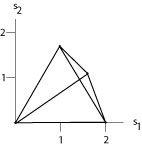
\includegraphics[height=2in]{2_tetra}}
\caption{Mapped tetrahedron of Solution \ref{op1_34}. \label{fig_tetra}}
\end{figure}

%%%%%%%%%%%%%%%%%%%%%%%%%%%%%%%%%%%%%%%%%%%%%%%%%%%%%%%%%%%%%%%%%%%%%%%%%%%%%%%%
\vspace{2mm}
\noindent {\bf Solution \ref{op1_35}}
We can write
\[
[s_1,s_2] = {{1}\over{\eee_3\cdot(\xx_0-\pp)+t\eee_3\cdot\vv}}[\eee_1\cdot(\xx_0-\pp)+t\eee_1\cdot\vv,\eee_2\cdot(\xx_0-\pp)+t\eee_2\cdot\vv]
\]
This means that $as_1+bs_2=c$ can be rewritten
\[
a(\eee_1\cdot(\xx_0-\pp)+t\eee_1\cdot\vv) + b(\eee_2\cdot(\xx_0-\pp)+t\eee_2\cdot\vv) - c(\eee_3\cdot(\xx_0-\pp)+t\eee_3\cdot\vv) = 0
\]
This holds for every $t$ if both these equations hold:
\[\matrix{
a(\eee_1\cdot(\xx_0-\pp)) &+ b(\eee_2\cdot(\xx_0-\pp)) &- c(\eee_3\cdot(\xx_0-\pp)) &= 0\cr
a\eee_1\cdot\vv &+ b\eee_2\cdot\vv &- c\eee_3\cdot\vv &=0\cr
}
\]
This is a system of two equations in three unknowns, $a$, $b$, and $c$. Such a system always has a non trivial solution (as we will see in
the following chapter.)

%%%%%%%%%%%%%%%%%%%%%%%%%%%%%%%%%%%%%%%%%%%%%%%%%%%%%%%%%%%%%%%%%%%%%%%%%%%%%%%%
\vspace{2mm}
\noindent {\bf Solution \ref{op1_36}}
In this case we want $\yy-\xx$ to point in the same direction as $\eee_3$ so
$\yy-\xx=\lambda\eee_3$. On the other hand $\yy$ lies on the plane of the
screen, so $\yy=\qq+s_1\eee_1+s_2\eee_2$. Therefore
\[
\qq-\xx+s_1\eee_1+s_2\eee_2=\lambda\eee_3.
\]
Now to find $s_1$ and $s_2$ take dot products with $\eee_1$ and $\eee_2$. This
yields
$s_1=-\eee_1\cdot(\qq-\xx)$ and $s_2=-\eee_2\cdot(\qq-\xx)$.


% \end{document}
